\chapter{Extending to agent-based model}

This chapter aims to explore an extension to the game described earlier.
The extension is based on the idea of an agent-based
model~\cite{de2014agent, fetta2012peter, knight2012modelling}.
What if the servers of the queueing system described in
Section~\ref{sec:queueing_section} could be treated as entities that could make
their own decisions?

The idea here is that servers could choose their own service rate so as to
maximise their own utility.
This would mean that the servers would be able to choose their own speed at
which they serve customers while the system is running.
Such decisions could be based on a number of factors, such as minimising the
number of customers in the system, minimising the proportion of patients lost
to the system, maximising their own idle time and so on.

The previous chapters are based on the assumption that hospitals and ambulances
play a non-cooperative game and act in their own self-interest.
Although this might be true in some cases, insights from ethnographic
studies~\cite{allen2004understanding} have shown that some cooperation and
empathy can be found among staff in such gaming environment.
The motivation for this chapter was initiated by these insights.

This chapter is structured in such a way that the first section describes a
state-dependent version of the queueing system described in
Section~\ref{sec:queueing_section}, the second section describes
a server-dependent variant and the third section combines them together and
formulate a reinforcement learning algorithm that works on finding the best
policies for the servers so that they can maximise their own utility.



\section{State-dependent variation}\label{sec:state_dependent}

This section focuses on creating a state-dependent variation of the queueing
system described in Section~\ref{sec:queueing_section}.
The state-dependent version is based on the idea that the speed of the servers
could be based on the number of individuals present in the system.

In the previous chapters of this thesis, the value of the service rate \(\mu\)
was set to a constant value.
For this variation of the model \(\mu\) will have a different value depending
on the number of individuals present in the two nodes of the queue.
In other words \(\mu\) will take a different value depending on the state
\((u, v)\) of which the system is in.
A parametric service rate \(\mu = \mu_{(u,v)}\) for a given \((u, v) \in S\) is
defined as follows:

\begin{equation}\label{eq:state_dependent_service_rate}
    \mu =
    \begin{cases}
        \mu_{(0,0)}, & \text{if } (u, v) = (0, 0) \\
        \mu_{(0,1)}, & \text{if } (u, v) = (0, 1) \\
        \quad \vdots & \qquad \quad \vdots \\
        \mu_{(M,N)}, & \text{if } (u, v) = (M, N)
    \end{cases}
\end{equation}

Consider an example of the queueing system described in
Section~\ref{sec:queueing_section} where the number of servers is set to
\(C = 1\), the threshold is set to \(T = 1\), node 1 capacity is \(N = 2\) and
node 2 capacity is \(M = 1\).
Figure~\ref{fig:state_dependent_markov_example} shows the state-dependent
Markov chain model of the queueing system.

\begin{figure}[H]
    \centering
    \begin{tikzpicture}[-, node distance = 2cm, auto]
\node[state] (u0v0) {(0,0)};
\node[state, right=of u0v0] (u0v1) {(0,1)};
\draw[->](u0v0) edge[bend left] node {\( \Lambda \)} (u0v1);
\draw[->](u0v1) edge[bend left] node {\( \mu_{(0,1)} \)} (u0v0);
\node[state, below=of u0v1] (u1v1) {(1,1)};
\draw[->](u0v1) edge[bend left] node {\( \lambda_2 \)} (u1v1);
\draw[->](u1v1) edge[bend left] node {\( \mu_{(1,1)} \)} (u0v1);
\node[state, right=of u0v1] (u0v2) {(0,2)};
\draw[->](u0v1) edge[bend left] node {\( \lambda_1 \)} (u0v2);
\draw[->](u0v2) edge[bend left] node {\( \mu_{(0,2)} \)} (u0v1);
\node[state, right=of u1v1] (u1v2) {(1,2)};
\draw[->](u1v1) edge[bend left] node {\( \lambda_1 \)} (u1v2);
\draw[->](u1v2) edge[bend left] node {\( \mu_{(1,2)} \)} (u1v1);
\draw[->](u0v2) edge node {\( \lambda_2 \)} (u1v2);
\end{tikzpicture}
    \caption{Markov chain example with \(C=1, T=1, N=2, M=1\)}
    \label{fig:state_dependent_markov_example}
\end{figure}

Consider the following value of \(\mu\) for the Markov chain model shown in
Figure~\ref{fig:state_dependent_markov_example}.

\begin{equation*}
    \mu =
    \begin{cases}
        \mu_{(0, 0)}, \text{ if } (u, v) = (0, 0) \\
        \mu_{(0, 1)}, \text{ if } (u, v) = (0, 1) \\
        \mu_{(0, 2)}, \text{ if } (u, v) = (0, 2) \\
        \mu_{(1, 1)}, \text{ if } (u, v) = (1, 1) \\
        \mu_{(1, 2)}, \text{ if } (u, v) = (1, 2)
    \end{cases}
\end{equation*}



\subsection{Implementation}

The state-dependent variation of the queueing system was implemented using the
python library \texttt{ciw}~\cite{ciwpython} only on the Discrete Event
Simulation (DES) version of the queueing model described in
Section~\ref{sec:discrete_event_simulation}.
All the code used to implement the state-dependent variation of the queueing
system is archived at~\cite{ambulance_game_github_repo} and developed openly on
GitHub.
More details on the code can be found in
Appendix~\ref{appendix:ambulance_game}.
The \texttt{ciw} library is structured in a way that allows the user to create
their own class for the service time distribution.
This class must inherit from the \texttt{ciw.dists.Distribution} class and
implement the \texttt{\_\_init\_\_} and \texttt{sample} methods.
The code snippet in~\ref{lst:state_dependent_class} shows the implementation of
the state-dependent service time distribution class.

\begin{lstlisting}[
    style=pystyle,
    caption={State-dependent service time distribution class.},
    label={lst:state_dependent_class}
]
>>> import ciw
>>> class StateDependentExponential(
...     ciw.dists.Distribution
... ):
...     def __init__(self, rates):
...         self.rates = rates
... 
...     def sample(self, t=None, ind=None):
...         """
...         This method is used to sample the service time for an
...         individual based on the current state
...         """
...         state = (
...             len(ind.simulation.nodes[1].individuals[0]),
...             len(ind.simulation.nodes[2].individuals[0]),
...         )
...         is_invalid_state = (
...             state[0] > 0 and state[1] < ind.simulation.threshold
...         )
...         if is_invalid_state:
...             state = (state[0] - 1, state[1] + 1)
...         rate = self.rates[state]
...         return random.expovariate(rate)
    
\end{lstlisting}

The function \texttt{simulate\_model} described in
Section~\ref{sec:discrete_event_simulation} takes \texttt{mu} as one of its
arguments.
If \texttt{mu} is set to a dictionary, with keys the states of the system and
values the service rate for each state (as shown in code
snippet~\ref{lst:state_dependent_example}), the service
distribution that will be
used in \texttt{ciw} will be a \texttt{StateDependentExponential} object.
The following code shows the implementation of the
\texttt{simulate\_model} function for the state-dependent variation of the
queueing system.

\begin{lstlisting}[
    style=pystyle,
    caption={Example of the state-dependent variation of the queueing system.},
    label={lst:state_dependent_example},
]
>>> import ambulance_game as abg
>>> import ciw
>>> import numpy as np
>>>
>>> lambda_1 = 1
>>> lambda_2 = 1
>>> num_of_servers = 1
>>> threshold = 1
>>> system_capacity = 2
>>> buffer_capacity = 1
>>> runtime = 1000
>>> seed_num = 0
>>>
>>> Q = abg.simulation.simulate_model(
...     lambda_1=lambda_1,
...     lambda_2=lambda_2,
...     mu={(0, 0): 2, (0, 1): 3, (0, 2): 4, (1, 1): 4, (1, 2): 5},
...     num_of_servers=num_of_servers,
...     threshold=threshold,
...     seed_num=seed_num,
...     system_capacity=system_capacity,
...     buffer_capacity=buffer_capacity,
...     runtime=runtime,
... )
>>> mean_waiting_time = np.mean([w.waiting_time for w in Q.get_all_records()])
>>> np.round(mean_waiting_time, 8)
0.06028274

\end{lstlisting}


\section{Server-dependent variation}\label{sec:server_dependent}

This section describes the creation of the server-dependent variation of the
queueing system described in Section~\ref{sec:queueing_section}.
The server-dependent model has a similar structure as the state-dependent model
described in Section~\ref{sec:state_dependent}.
In this variation each server has its own service rate.

Similar to Section~\ref{sec:state_dependent} the server-dependent variation of
the parametric service rate \(\mu = \mu_i\) for a given
\(i \in {1, 2, \dots, C}\) (where \(C\) is the number of servers) is defined as
follows:

\begin{equation}\label{eq:server_dependent_service_rate}
    \mu =
    \begin{cases}
        \mu_1, & \text{for server } 1 \\
        \mu_2, & \text{for server } 2 \\
        \quad \vdots & \qquad \quad \vdots \\
        \mu_C, & \text{for server } C
    \end{cases}
\end{equation}

Consider an example of the queueing system described in
Section~\ref{sec:queueing_section} where the number of servers is set to
\(C = 4\), the threshold is set to \(T = 1\), node 1 capacity is \(N = 2\) and
node 2 capacity is \(M = 1\).
The value of the service rate \(\mu\) for the DES model can take the following
values:

\begin{equation*}
    \mu =
    \begin{cases}
        \mu_1, & \text{for server } 1 \\
        \mu_2, & \text{for server } 2 \\
        \mu_3, & \text{for server } 3 \\
        \mu_4, & \text{for server } 4
    \end{cases}
\end{equation*}



\subsection{Implementation}

The server-dependent variation of the queueing system is implemented in a
similar way as the state-dependent implementation.
Using the python library \texttt{ciw} the server-dependent service time
distribution is defined as a class that inherits from the
\texttt{ciw.dists.Distribution} class.
The class is defined as follows:

\begin{lstlisting}[style=pystyle]
>>> import random
>>> import ciw
>>> class ServerDependentExponential(
...     ciw.dists.Distribution
... ):
...     def __init__(self, rates):
...         self.rates = rates
... 
...     def sample(self, t=None, ind=None):
...         """
...         This method is used to sample the service time for an individual based
...         on the server that the individual is assigned to
...         """
...         server = ind.server.id_number
...         rate = self.rates[server]
...         return random.expovariate(rate)
    
\end{lstlisting}

Similar to the state-dependent implementation, the function
\texttt{simulate\_model} from Section~\ref{sec:discrete_event_simulation} is
used to simulate the server-dependent variation of the queueing system.
The main difference from the state-dependent case is that the service rate
\(\mu\) is now a dictionary with the server's id as the key and the service
rate of that server as the value.

\begin{lstlisting}[style=pystyle]
>>> import ambulance_game as abg
>>> import ciw
>>> import numpy as np
>>>
>>> lambda_1 = 1
>>> lambda_2 = 1
>>> num_of_servers = 4
>>> threshold = 1
>>> system_capacity = 8
>>> buffer_capacity = 2
>>> runtime = 1000
>>> seed_num = 0
>>>
>>> Q = abg.simulation.simulate_model(
...     lambda_1=lambda_1,
...     lambda_2=lambda_2,
...     mu={
...         1: 0.5,
...         2: 0.5,
...         3: 1.0,
...         4: 1.5,
...     },
...     num_of_servers=num_of_servers,
...     threshold=threshold,
...     seed_num=seed_num,
...     system_capacity=system_capacity,
...     buffer_capacity=buffer_capacity,
...     runtime=runtime,
... )
>>> mean_waiting_time = np.mean([w.waiting_time for w in Q.get_all_records()])
>>> np.round(mean_waiting_time, 8)
0.02668017

\end{lstlisting}



\section{State and server-dependent model}\label{sec:state_server_dependent_model}

In addition, the final variation of the queueing model is one that is both
state and server-dependent.
That is, for each server and for each state there is a different service rate.
In other words, each server can have a different service rate for every
possible scenario that the system can be in.

The new service rate \(\mu\) that will be used in this scenario is defined as
a combination of equations~(\ref{eq:state_dependent_service_rate})
and~(\ref{eq:server_dependent_service_rate}) where:

\begin{equation}\label{eq:state_server_dependent_service_rate}
    \mu =
    \begin{cases}
        \mu_{1, (0,0)}, & \text{for server } 1 \text{ if } (u, v) = (0, 0) \\
        \mu_{1, (0,1)}, & \text{for server } 1 \text{ if } (u, v) = (0, 1) \\
        \quad \vdots & \qquad \qquad \vdots \\
        \mu_{1, (N,M)}, & \text{for server } 1 \text{ if } (u, v) = (M, N) \\
        \mu_{2, (0,0)}, & \text{for server } 2 \text{ if } (u, v) = (0, 0) \\
        \mu_{2, (0,1)}, & \text{for server } 1 \text{ if } (u, v) = (0, 1) \\
        \quad \vdots & \qquad \qquad \vdots \\
        \mu_{2, (N,M)}, & \text{for server } 2 \text{ if } (u, v) = (M, N) \\
        \quad \vdots & \qquad \qquad \vdots \\
        \mu_{C, (0,0)}, & \text{for server } C \text{ if } (u, v) = (0, 0) \\
        \mu_{C, (0,1)}, & \text{for server } C \text{ if } (u, v) = (0, 1) \\
        \quad \vdots & \qquad \qquad \vdots \\
        \mu_{C, (N,M)}, & \text{for server } C \text{ if } (u, v) = (M, N)
    \end{cases}
\end{equation}

Consider an example where the number of servers is set to \(C = 2\), the
threshold is set to \(T = 1\), node 1 capacity is \(N = 3\) and node 2 capacity
is \(M = 1\).
For this particular example the possible values that \(\mu\) can take shown
by equation~(\ref{eq:state_server_dependent_service_rate_example}).

\begin{equation}\label{eq:state_server_dependent_service_rate_example}
    \mu =
    \begin{cases}
        \mu_{1, (0,0)}, & \text{for server } 1 \text{ if } (u, v) = (0, 0) \\
        \mu_{1, (0,1)}, & \text{for server } 1 \text{ if } (u, v) = (0, 1) \\
        \mu_{1, (0,2)}, & \text{for server } 1 \text{ if } (u, v) = (0, 2) \\
        \mu_{1, (0,3)}, & \text{for server } 1 \text{ if } (u, v) = (0, 3) \\
        \mu_{1, (1,0)}, & \text{for server } 1 \text{ if } (u, v) = (1, 0) \\
        \mu_{1, (1,1)}, & \text{for server } 1 \text{ if } (u, v) = (1, 1) \\
        \mu_{1, (1,2)}, & \text{for server } 1 \text{ if } (u, v) = (1, 2) \\
        \mu_{1, (1,3)}, & \text{for server } 1 \text{ if } (u, v) = (1, 3) \\
        \mu_{2, (0,0)}, & \text{for server } 2 \text{ if } (u, v) = (0, 0) \\
        \mu_{2, (0,1)}, & \text{for server } 2 \text{ if } (u, v) = (0, 1) \\
        \mu_{2, (0,2)}, & \text{for server } 2 \text{ if } (u, v) = (0, 2) \\
        \mu_{2, (0,3)}, & \text{for server } 2 \text{ if } (u, v) = (0, 3) \\
        \mu_{2, (1,0)}, & \text{for server } 2 \text{ if } (u, v) = (1, 0) \\
        \mu_{2, (1,1)}, & \text{for server } 2 \text{ if } (u, v) = (1, 1) \\
        \mu_{2, (1,2)}, & \text{for server } 2 \text{ if } (u, v) = (1, 2) \\
        \mu_{2, (1,3)}, & \text{for server } 2 \text{ if } (u, v) = (1, 3)
    \end{cases}
\end{equation}


\subsection{Implementation}

The implementation of the state and server-dependent model is the
combination of the state-dependent and server-dependent models' implementation.
Once again the implementation is done using the python library \(\texttt{ciw}\)
library.
The distribution for the state and server-dependent model is defined as a
class that inherits from the \texttt{ciw}'s class
\texttt{ciw.dists.Distribution}.
Note that as opposed to the classes defined earlier an additional method id
defined in this class.
Method \texttt{update\_server\_attributes} adds additional attributes to the
server objects to allow for further analysis of each server's performance.

\begin{lstlisting}[style=pystyle]
>>> import random
>>> import ciw
>>> class StateServerDependentExponential(
...     ciw.dists.Distribution
... ):
...     def __init__(self, rates):
...         self.simulation = None
...         self.rates = rates
... 
...     def sample(self, t=None, ind=None):
...         """
...         This method is used to sample the service time for an individual based
...         on the current state and the server that the individual is assigned to.
...         The following steps are being taken:
...             1. Find the server
...             2. Find the state
...             3. Check if the state is valid. Note that there are some cases where
...                 the visited state is not valid. These are the cases where the
...                 state `(u, T-1)` is visited where `u > 0`. This is meant to be
...                 an unreachable state. In such case remap the state to `(u+1, T)`
...             4. Get the service rate for that server and state
...             5. Sample the service time
...             6. Update any possible attributes for the server
...         """
...         server = ind.server.id_number
...         state = (
...             len(ind.simulation.nodes[1].individuals[0]),
...             len(ind.simulation.nodes[2].individuals[0]),
...         )
...         is_invalid_state = state[0] > 0 and state[1] < ind.simulation.threshold
...         if is_invalid_state:
...             state = (state[0] - 1, state[1] + 1)
...         rate = self.rates[server][state]
...         service_time = random.expovariate(rate)
...         self.update_server_attributes(ind, service_time)
...         return service_time
... 
...     def update_server_attributes(self, ind, service_time):
...         """
...         Updates the server's attributes
...         """
...         if hasattr(ind.server, "served_inds"):
...             ind.server.served_inds.append(self.simulation.current_time)
...         else:
...             ind.server.served_inds = [self.simulation.current_time]
... 
...         if hasattr(ind.server, "service_times"):
...             ind.server.service_times.append(service_time)
...         else:
...             ind.server.service_times = [service_time]

\end{lstlisting}

Now consider an example where the number of servers is set to \(C = 2\), the
threshold is set to \(T = 1\), node 1 capacity is \(N = 3\) and node 2 capacity
is \(M = 1\).
Let the service rates be defined in such a way where:

\begin{enumerate}
    \item Server 1's service rate is \(0.5\) whenever there are less than two
    individuals in the entire system, otherwise the service rate is \(1\).
    \item Server 2's service rate is \(0.7\) whenever there are less than three
    individuals in the entire system, otherwise the service rate is \(1.5\).
\end{enumerate}

The following code snippet shows how to define the model and run the simulation
for \(1000\) time units.

\begin{lstlisting}[style=pystyle]
>>> import ambulance_game as abg
>>> import numpy as np
>>>
>>> lambda_1 = 1
>>> lambda_2 = 1
>>> num_of_servers = 2
>>> threshold = 1
>>> system_capacity = 3
>>> buffer_capacity = 1
>>> runtime = 1000
>>> seed_num = 0
>>> 
>>> all_states = abg.markov.build_states(
...     threshold=threshold,
...     system_capacity=system_capacity,
...     buffer_capacity=buffer_capacity
... )
>>> mu = {k: {} for k in range(1, num_of_servers + 1)}
>>> mu[1] = {(u, v): 0.5 if u + v < 2 else 1 for u, v in all_states}
>>> mu[2] = {(u, v): 0.7 if u + v < 3 else 1.5 for u, v in all_states}
>>>
>>> Q = abg.simulation.simulate_model(
...     lambda_1=lambda_1,
...     lambda_2=lambda_2,
...     mu=mu,
...     num_of_servers=num_of_servers,
...     threshold=threshold,
...     seed_num=seed_num,
...     system_capacity=system_capacity,
...     buffer_capacity=buffer_capacity,
...     runtime=runtime,
... )
>>> for srv, mean_service_time in enumerate([
...     np.round(np.mean(s.service_times), 8)
...     for s in Q.nodes[2].servers
... ]):
...     print(f"Server {srv + 1}:", mean_service_time)
Server 1: 1.79718861
Server 2: 0.87253758

\end{lstlisting}

Note that, in the implementation above the individuals are paired with a server
in an ``unfair'' way since the default behaviour of \texttt{ciw} does not
focus on the fairness of server allocation.
Server 1 is always assigned an individual if they are free, while Server 2 is
only assigned an individual if Server 1 is busy.
For the purposes of this project though, it is important to have a more
``fair'' allocation of individuals to servers.
This can be done by using the server\_priority\_function argument of the
\texttt{simulate\_model} function.

\begin{lstlisting}[style=pystyle]
>>> Q = abg.simulation.simulate_model(
...     lambda_1=lambda_1,
...     lambda_2=lambda_2,
...     mu=mu,
...     num_of_servers=num_of_servers,
...     threshold=threshold,
...     seed_num=seed_num,
...     system_capacity=system_capacity,
...     buffer_capacity=buffer_capacity,
...     runtime=runtime,
...     server_priority_function=lambda srv, ind: random.random()
... )
>>> for srv, mean_service_time in enumerate([
...     np.round(np.mean(s.service_times), 8)
...     for s in Q.nodes[2].servers
... ]):
...     print(f"Server {srv + 1}:", mean_service_time)
Server 1: 1.31071177
Server 2: 1.02142722

\end{lstlisting}


\subsection{Game theoretic model}

In fact the state and server dependent model can be used in the game theoretic
model described from Section~\ref{sec:game_theoretic_model}.
Although, since the state and server dependent model variant of the queueing
theoretic model is only implemented using Discrete Event Simulation (DES) it is
not possible to use the Markov chain model here.
Thus, the implementation of the game was modified so that it can be used with
the DES model as well.
More details on the code can be found in appendix~\ref{appendix:ambulance_game}.
At its core the only metric that is needed from the Markov model are the
performance measures of the queue (blocking time and proportion of individuals
within target) which can also be obtained using the DES model.
Consequently, the payoff matrices can be calculated using these performance
measures.

Something that needs to be taken into consideration here is whether the results
of the game are the same when using the DES model and the Markov chain model.
In fact using the DES approach several other parameters are introduced that
can affect the results of the game.
Such parameters are the runtime, the warm up time and the cooldown time of the
simulation.
The one that is of most interest here is the runtime.

Consider a game with the following parameters:

\begin{multicols}{3}
    \begin{itemize}
        \item \( \lambda_1^{(1)} = 2 \)
        \item \( \mu^{(1)} = 2 \)
        \item \( C^{(1)} = 2 \)
        \item \( N^{(1)} = 6 \)
        \item \( M^{(1)} = 2 \)

        \columnbreak
        \item \( \lambda_1^{(2)} = 2 \)
        \item \( \mu^{(2)} = 2 \)
        \item \( C^{(2)} = 2 \)
        \item \( N^{(2)} = 6 \)
        \item \( M^{(2)} = 2 \)

        \columnbreak
        \item \( \lambda_2 = 2 \)
        \item \( t = 2 \)
        \item \( \alpha = 0.2 \)
        \item \( \hat{P} = 0.95 \)
    \end{itemize}    
\end{multicols}

For a complete description of parameter notations see
Section~\ref{sec:game_players_and_parameters}.
Figure~\ref{fig:game_des_markov_baseline} shows the asymmetric replicator
dynamics run of the game when the payoff matrices are calculated using the
Markov chain model.

\begin{figure}[ht]
    \centering
    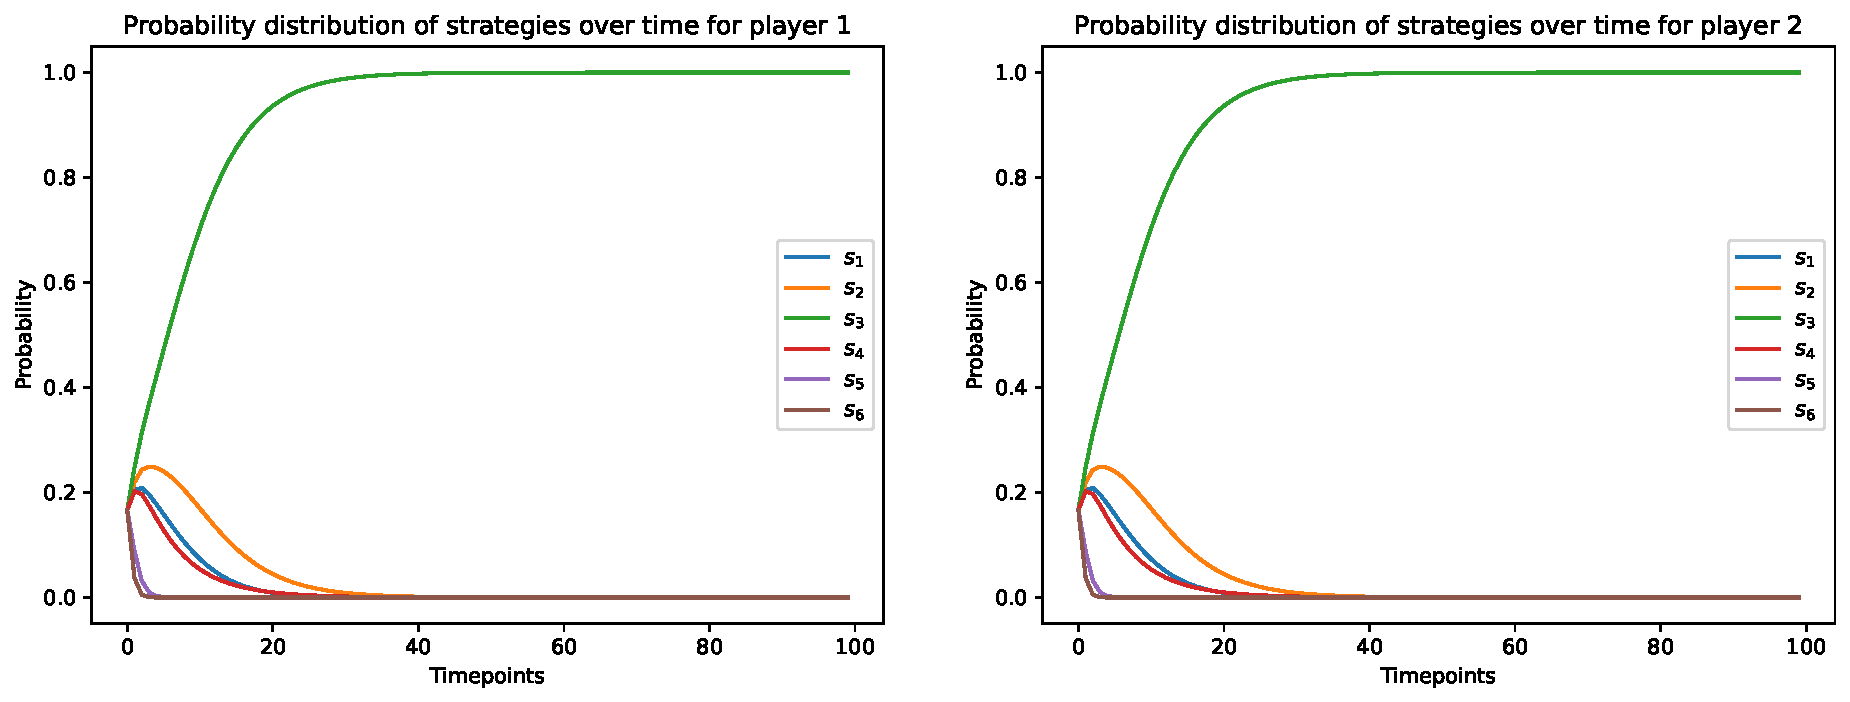
\includegraphics[width=0.8\textwidth]{chapters/06_agent_based_extension/Bin/game_model_with_des/game_markov_baseline.pdf}
    \caption{Asymmetric replicator dynamics algorithm run on the game obtained
    from the Markov chain model.}
    \label{fig:game_des_markov_baseline}
\end{figure}

It can be seen that both player end up playing strategy \(s_3\) which is the
choosing a threshold of \((T^{(1)} = 3, T^{(2)} = 3)\).
Figures~\ref{fig:game_des_runtime_300}, \ref{fig:game_des_runtime_500} and
\ref{fig:game_des_runtime_1000} show the asymmetric replicator dynamics run of
the game when the payoff matrices are calculated using the DES model with
different runtimes.
More specifically, the runtime of the DES model is set to \(300\), \(500\) and
\(1000\) time units respectively.

\begin{figure}[H]
    \centering
    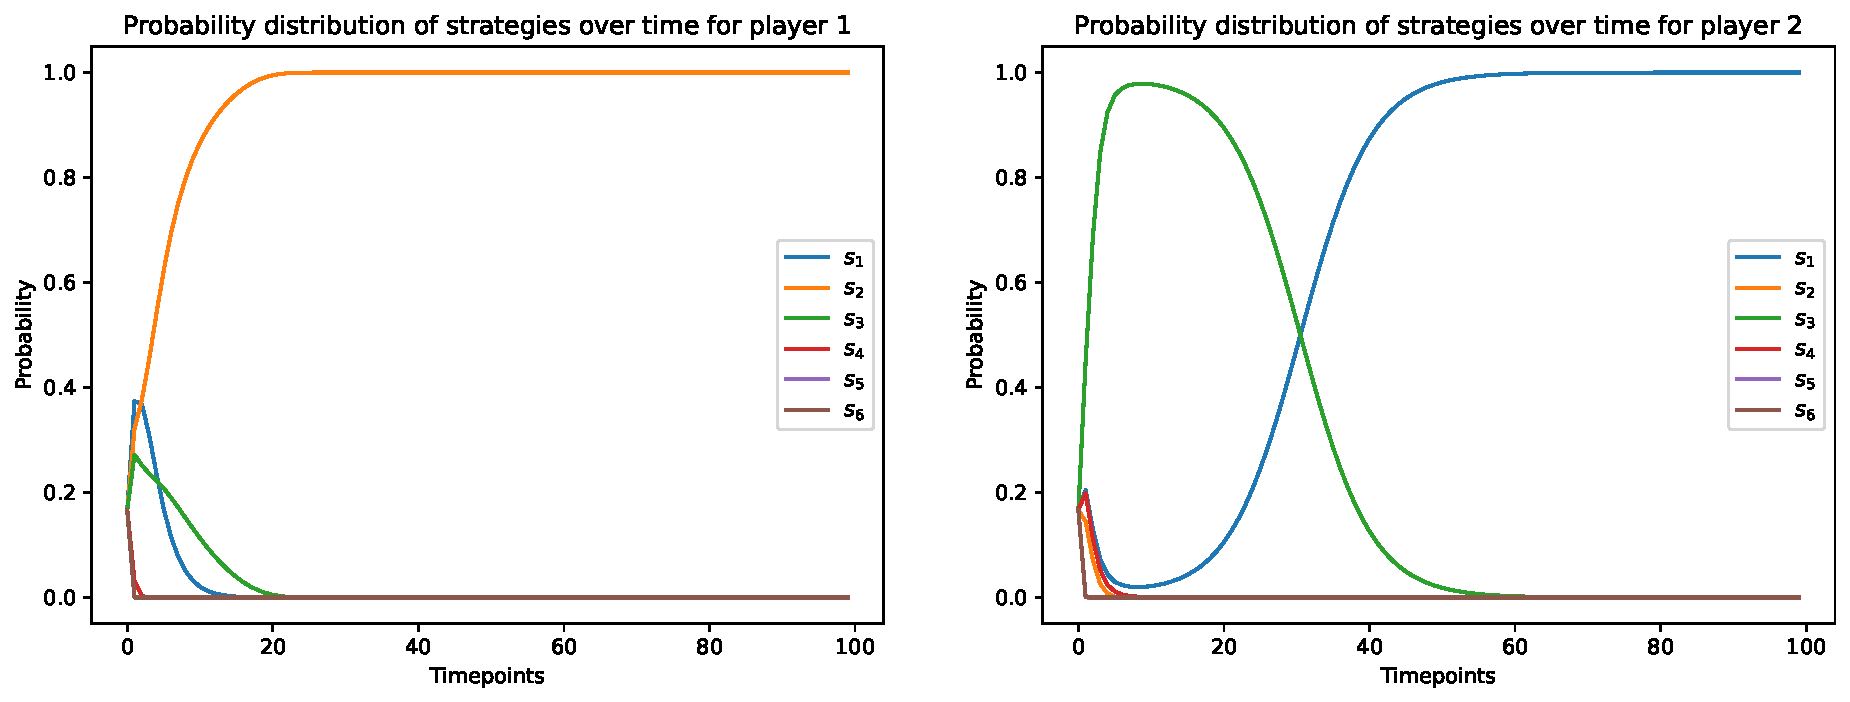
\includegraphics[width=0.8\textwidth]{chapters/06_agent_based_extension/Bin/game_model_with_des/game_simulation_300.pdf}
    \caption{Asymmetric replicator dynamics algorithm run on the game obtained
    from the DES model using a runtime of \(300\) time units.}
    \label{fig:game_des_runtime_300}
\end{figure}

\begin{figure}[H]
    \centering
    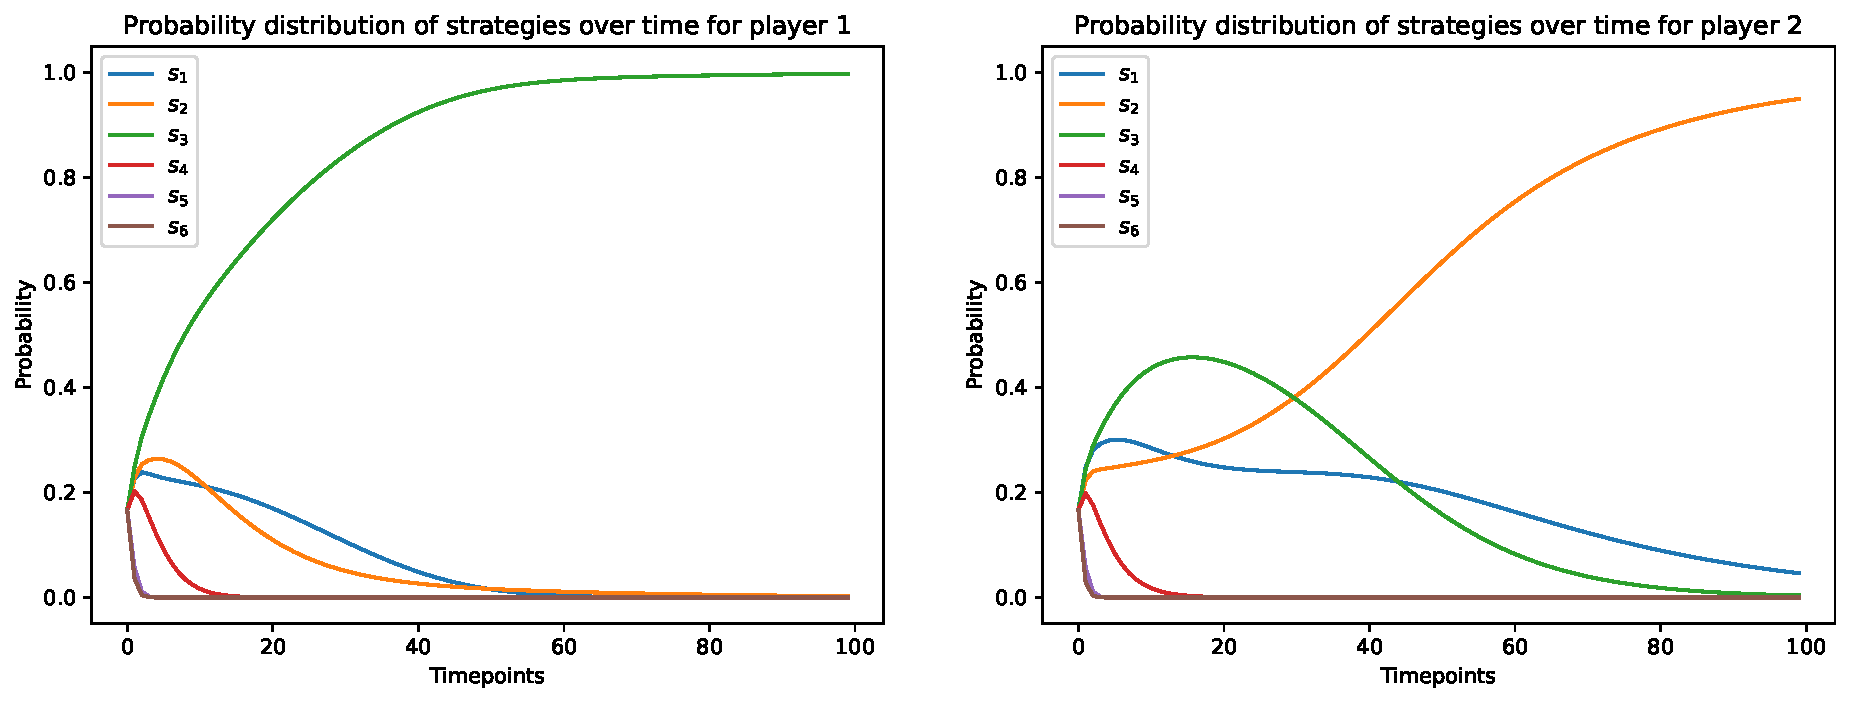
\includegraphics[width=0.8\textwidth]{chapters/06_agent_based_extension/Bin/game_model_with_des/game_simulation_500.pdf}
    \caption{Asymmetric replicator dynamics algorithm run on the game obtained
    from the DES model using a runtime of \(500\) time units.}
    \label{fig:game_des_runtime_500}
\end{figure}

\begin{figure}[H]
    \centering
    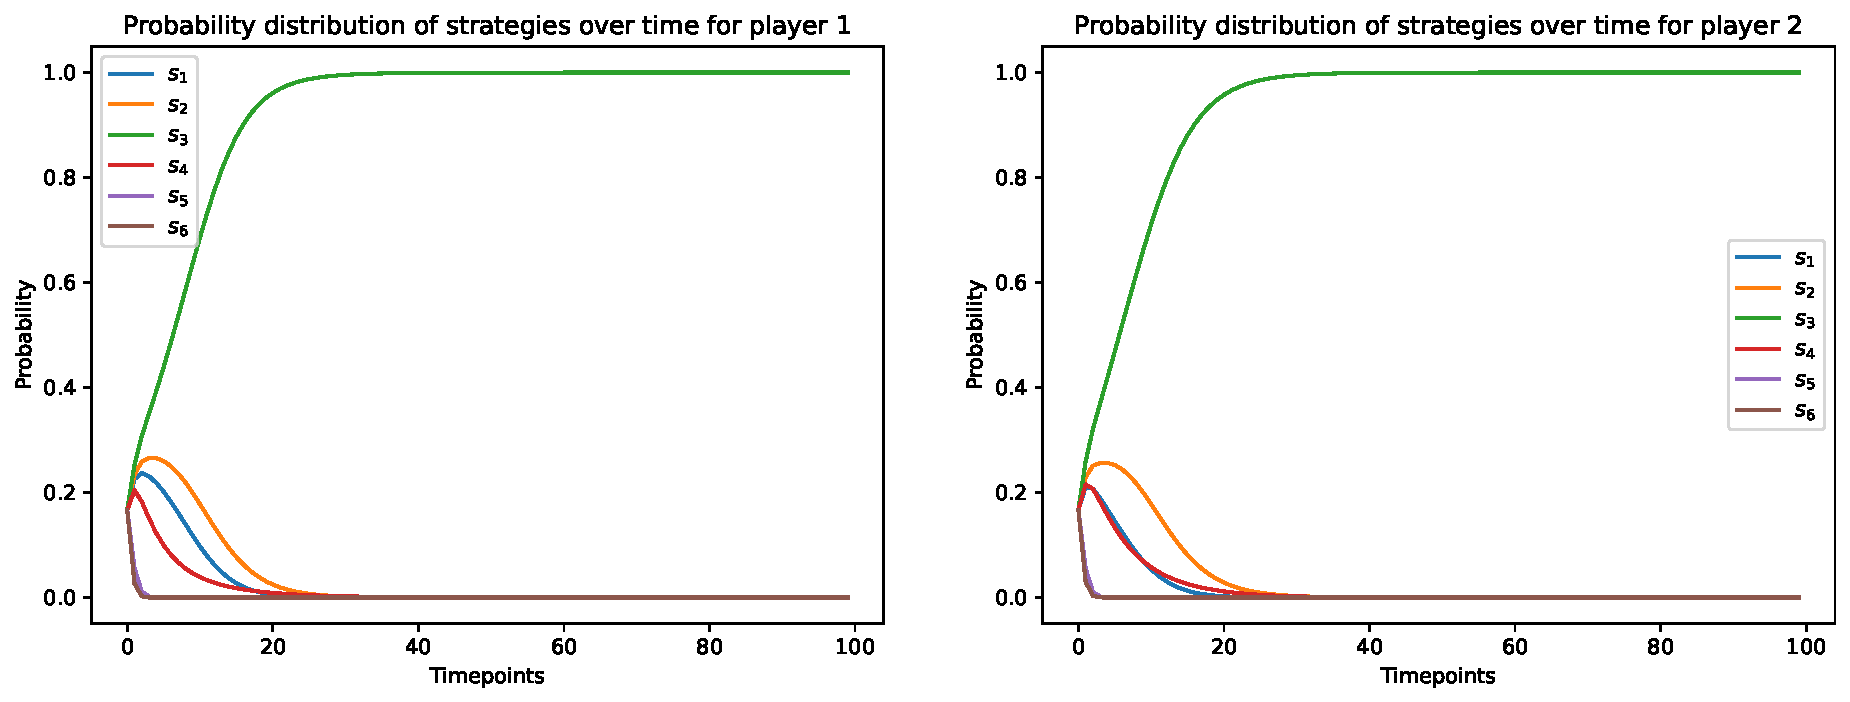
\includegraphics[width=0.8\textwidth]{chapters/06_agent_based_extension/Bin/game_model_with_des/game_simulation_1000.pdf}
    \caption{Asymmetric replicator dynamics algorithm run on the game obtained
    from the DES model using a runtime of \(1000\) time units.}
    \label{fig:game_des_runtime_1000}
\end{figure}

By observing the asymmetric replicator dynamics run of the game with the DES
model when using different runtimes, it can be noticed that the results from
using a runtime of \(300\) time units and a runtime of \(500\) time units are
different from the ones obtained using the Markov chain model.
However, the resultant strategies from using a runtime of \(1000\) time units
are the same as the ones obtained using the Markov chain model.
This is due to the fact that the runtime of the DES model needs to be long
enough for the simulation to reach a steady state.
For this particular example, it seems that a runtime of \(1000\) time units is
sufficient.


Having found a reasonable runtime for the DES model, the state and server
dependent distribution of the service rate can be used in the game theoretic
model.
Consider a small change to the parameter values defined earlier, where the
service rate is now state and server dependent.
Let the service rate for queueing system \(1\) be \(\mu^{(1)} = 6\) only for
server \(1\) if there are \(4\) or more individuals individuals in the system
and \(\mu^{(1)} = 2\) otherwise.
Additionally, let the service rate for queueing system \(2\) be
\(\mu^{(2)} = 8\) only for server \(1\) if there are \(3\) or more
individuals in node 1 and \(\mu^{(2)} = 2\) otherwise.
In other words the service rate is now defined as:

\begin{align}
    \mu_1 =
    \begin{cases}
        6, & \text{if server id \(= 1\) and } u_1 + v_1 \geq 4 \\
        2, & \text{otherwise}
    \end{cases} \\
    \mu_2 =
    \begin{cases}
        8, & \text{if server id \(= 1\) and } u_1 \geq 3 \\
        2, & \text{otherwise}
    \end{cases}
\end{align}

The game theoretic model is then run using the DES model with a runtime of
\(3000\) time units.
Figure~\ref{fig:game_server_state_dependen_example} shows the asymmetric
replicator dynamics run of the game when the payoff matrices are calculated
using the DES model with this new service rate distribution.

\begin{figure}[H]
    \centering
    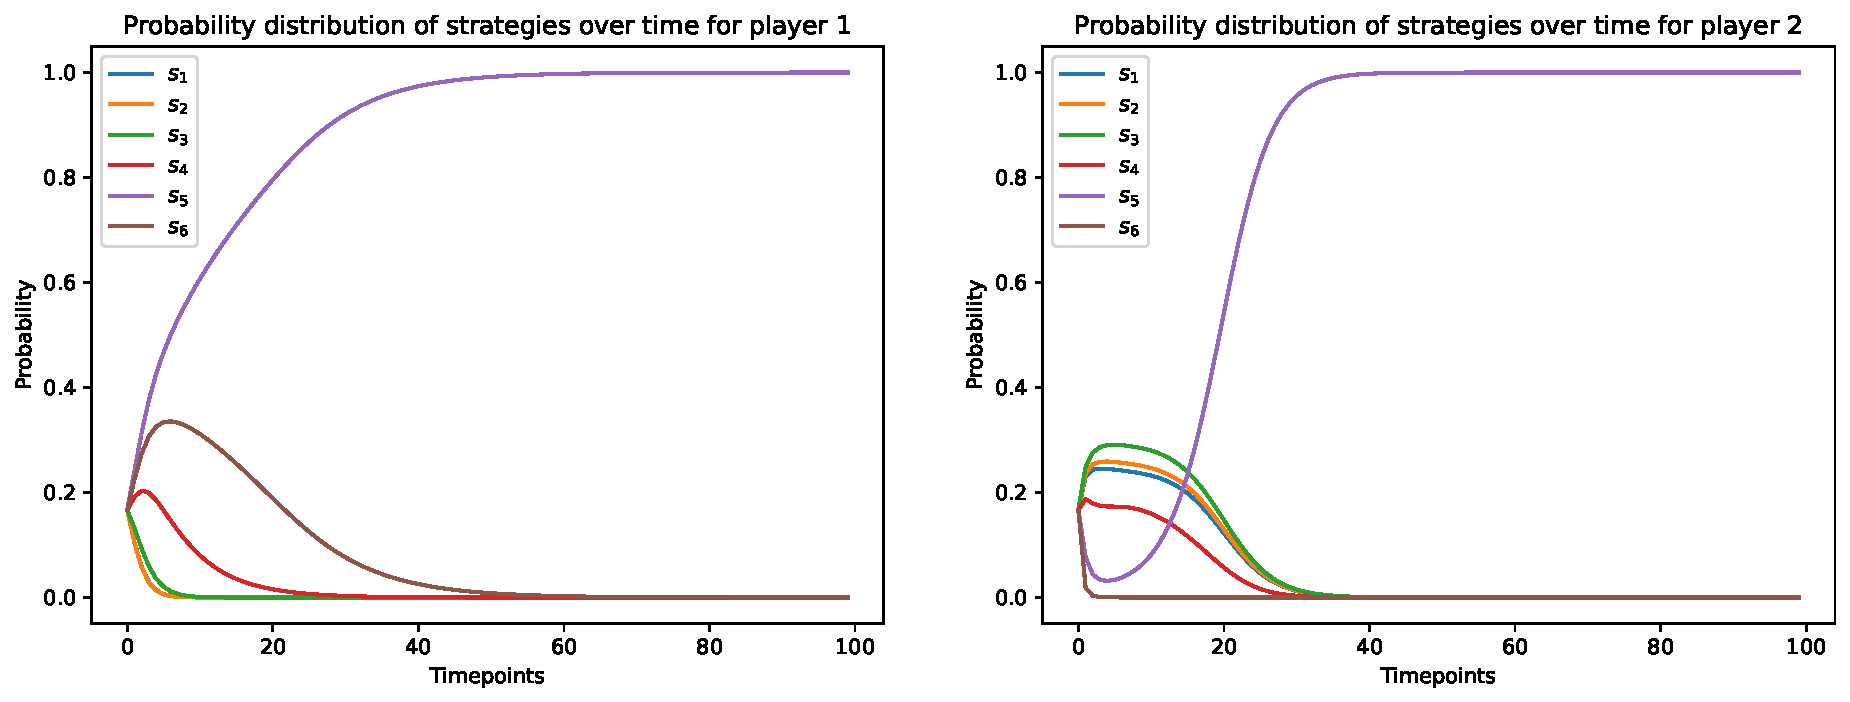
\includegraphics[width=0.8\textwidth]{chapters/06_agent_based_extension/Bin/game_model_with_des/game_server_state_dependent_3000.pdf}
    \caption{Asymmetric replicator dynamics algorithm run on the game obtained
    from the DES model using a runtime of \(3000\) time units and a state and
    server dependent service rate.}
    \label{fig:game_server_state_dependen_example}
\end{figure}

It can be seen that the outcome of the game is different than before.
Player \(1\) chooses to play strategy \(s_5\) and player \(2\) also ends up
playing strategy \(s_5\).
That corresponds to choosing a threshold of \(T^{(1)} = 5\) and a threshold of
\(T^{(2)} = 5\).
The change in the service distribution made server \(1\) of queueing system
\(1\) and server \(1\) of queueing system \(2\) work faster when their
corresponding system was getting busier.
This change in the service rate distribution made the queueing systems
increase their thresholds in the game, and thus block less type \(2\)
individuals at node \(1\).
Refer to Figure~\ref{fig:diagram_of_queueing_system} for a visual
representation of the types of individuals and the nodes of the queueing
systems. 



\section{The agent-based model}\label{sec:agent_based_model}

Section~\ref{sec:state_server_dependent_model} describes an extension to the
queueing system described in Section~\ref{sec:queueing_section} that allows
each server to have their own service rate for every possible state of the
system.
In this section, an agent-based model is proposed where servers are considered
as agents that can make their own decisions.
The idea is that every agent in the system can choose their own service rate
based on some utility function that they aim to maximise.
This would mean that the servers would be able to choose and update their own
speed at which they serve individuals while the system is running.
Such decisions could be based on a number of factors, such as minimising the
number of patients in the system, minimising the proportion of patients lost
to the system, maximising their own idle time and so on.

\subsection{Utility functions}

Utility functions are a way of quantifying how ``happy'' an agent is with the
current condition of the system~\cite{fishburn1970utility, fishburn1968utility}.
Each agent in the system can have their own utility function that they aim to
maximise.
In a realistic scenario, these utility functions could be based in a number of
factors, where each agent can have a different weight for each factor.

At the end of the simulation run there are some key performance measures that
can be extracted to quantify the performance of the overall system and each
server individually.
Table~\ref{tab:server_agents_performance_measures} shows these measures that
will then be used to formulate the utility functions.

\begin{table}[htbp]
    \centering
    \caption{Performance measures that could affect each agent's utility}
    \label{tab:server_agents_performance_measures}
    \begin{tabular}{|c|c|}
        \hline
        \textbf{Notation} & \textbf{Description} \\
        \hline
        \hline
        \(I\) & Total number of individuals (both served and lost) \\
        \hline
        \(I_s\) & Number of served individuals \\
        \hline
        \(I_L\) & Number of individuals that are lost due to the system being
        full \\
        \hline
        \(I_s^{(k)}\) & All individuals served by server \(k\) \\
        \hline
        \(R\) & Overall runtime of the simulation \\
        \hline
        \(B^{(k)}\) & Busy time of server \(k\) \\
        \hline
        \(R - B^{(k)}\) & Idle time of server \(k\) \\
        \hline
        \(\bar{\mu}^{(k)}\) & Mean service rate of server \(k\) \\
        \hline
        \(\bar{m}^{(k)}\) & Mean service time of server \(k\) \\
        \hline
    \end{tabular}
\end{table}

Note that the difference between the mean service rate and the mean service
time is that the mean service rate is the average out of all the service rates
for every state \((u, v)\) with no particular weight given to any of them.
In contrast, the mean service time is the average of all the service times
that each server has experienced.
That means that if a particular state has not been visited by a server, then
the mean service time will not be affected by that state.

The above measures could be combined together in a number of ways to formulate
utility functions.
Some examples of utility functions that could be used are the following:

\begin{align}
    U_k^{(1)} &= e \, I_s^{(k)} + (1 - e) \, (R - B^{(k)})
    \label{eq:utility_1} \\
    U_k^{(2)} &= e \, \frac{I_s^{(k)}}{I_s} + (1 - e) \, \frac{R - B^{(k)}}{R}
    \label{eq:utility_2} \\
    U_k^{(3)} &= e \, \bar{m}^{(k)} + (1 - e) \, (R - B^{(k)})
    \label{eq:utility_3} \\
    U_k^{(4)} &= e \, \bar{\mu}^{(k)} + (1 - e) \, (R - B^{(k)})
    \label{eq:utility_4} \\
    U_k^{(5)} &= e \, \frac{I_s^{(k)}}{I_s} + (1 - e) \, \bar{m}^{(k)}
    \label{eq:utility_5} \\ 
    U_k^{(6)} &= e \, \frac{I_s^{(k)}}{I} + (1 - e) \, \frac{1}{\bar{m}^{(k)}}
    \label{eq:utility_6} \\
    U_k^{(7)} &= e \, \frac{I_s}{I} + (1 - e) \, \frac{R - B^{(k)}}{R}
    \label{eq:utility_7} \\
\end{align}

where \(U_k^{(i)}\) is utility \(i\) of server \(k\) and \(e\) is a parameter that
can be used to weight the importance of each measure.
For example, \(e = 0.5\) would mean that the two measures are equally important
for the agent.
Table~\ref{tab:utility_functions_description} gives a brief description of each
utility function.

\begin{table}[htbp]
\centering
\caption{Utility functions that can be used to measure each server's
happiness}
\label{tab:utility_functions_description}
\begin{tabular}{|c|c|}
    \hline
    \textbf{Utility function} & \textbf{Description} \\
    \hline
    \hline
    \(U_k^{(1)}\)   & Weighted average between the number of served \\ 
                    & individuals by server \(k\) and idle time of server \(k\) \\
    \hline
    \(U_k^{(2)}\)   & Weighted average between overall proportion of served \\
                    & individuals by server \(k\) and proportion of idle \\
                    & time of server \(k\) \\
    \hline
    \(U_k^{(3)}\)   & Weighted average between mean service time of \\
                    & server \(k\) and idle time of server \(k\) \\
    \hline
    \(U_k^{(4)}\)   & Weighted average between mean service rate of \\
                    & server \(k\) and idle time of server \(k\) \\
    \hline
    \(U_k^{(5)}\)   & Weighted average between proportion of served \\
                    & individuals by server \(k\) and mean service time of
                    server \(k\) \\
    \hline
    \(U_k^{(6)}\)   & Weighted average between proportion of served \\
                    & individuals by server \(k\) and inverse of mean \\
                    & service time of server \(k\) \\
    \hline
    \(U_k^{(7)}\)   & Weighted average between overall proportion of served \\
                    & individuals and proportion of idle time of server \(k\) \\
    \hline
\end{tabular}
\end{table}

\subsection{Case study}\label{sec:agent_based_case_study}

In this subsection, an empirical study is presented to show how the above
utility functions can be used to measure each server's ``happiness''.
The study builds upon the empirical study on the queueing system described
in~\cite{harper2020server}.
This subsection will use the same data set as in~\cite{harper2020server}, but
applied to the queueing system described in Section~\ref{sec:queueing_section}
and the agent-based model described in Section~\ref{sec:agent_based_model}.

In that study a set of data was collected from a large emergency department in
Wales, UK.
The data was collected over 6 months and contained information
on each patient that arrived at the emergency department.
Such information included the time of arrival, the time of service, the triage
category and the time of discharge.
The dataset consisted of \(4,832\) patients that were considered as ``urgent''.
In~\cite{harper2020server} it was shown that as the workload of the system
changed, the service times of the serves also changed.
In fact, low to moderate workload levels resulted in service times that were
lower than the service times experienced at high workload levels.

The system was modelled as a single-server queueing system with two service
speeds.
Arrivals follow a Poisson distribution with mean inter-arrival time
of \(92\) minutes, thus the arrival rate can be set to
\(\lambda = \frac{1}{92}\).
The service speed was partitioned into two distributions; one for low to
moderate workload levels and one for high workload levels.
The service speed for the low to moderate workload levels was found to follow
a lognormal distribution with a mean of \(86\) minutes and the service speed for
the high workload levels was found to follow a lognormal distribution
with a mean of \(62\) minutes.
Therefore, the service rates can be set to \(\mu_1 = \frac{1}{86}\) and
\(\mu_2 = \frac{1}{62}\).
It was observed that the slow service speed was used for when \(6\) or less
individuals were in the system and the fast service speed was used for when
\(7\) or more individuals were present. 

The above parameters were slightly modified so that they are applied to the
queueing system described in Section~\ref{sec:queueing_section}.
In essence, the queueing system is now a \(4\) server system and the arrival
rate is set to \(\lambda = 4 \times \frac{1}{92}\) and the two service speeds
stay the same.
In addition, the new arrival rate is now split into two distributions, one for
type 1 individuals and one for type 2 individuals.
Type 1 arrivals follow a Poisson distribution with mean inter-arrival time
of \(57.5\) minutes and type 2 arrivals follow a Poisson distribution with mean
inter-arrival time of \(38.3\) minutes.
Therefore, the arrival rates for type 1 and type 2 individuals are
\(\lambda_1 = \frac{1}{57.5}\) and \(\lambda_2 = \frac{1}{38.3}\) respectively.

Additionally, for this modified example the \(4\) servers fall into one of
three groups; experienced, moderate and intern.
In particular server \(1\) is an experienced server, server \(2\) and server
\(3\) are moderate servers and server \(4\) is an intern.
This means that server \(1\) has a slightly higher service rate than the other
servers and if they are available they will always be assigned the incoming
individual.
Servers \(2\) and \(3\) have the same service rate and if they are available
they may be assigned the incoming individual with an equal probability.
Finally, server \(4\) has the lowest service rate and they will only be
assigned the incoming individual if the other servers are unavailable.
More specifically, the service rates for the ``experienced'' server is
multiplied by a factor of \(1.2\) and the service rates for the ``intern''
server is multiplied by a factor of \(0.8\), while the ``moderate'' servers
stay unchanged.
Whilst this might not be a realistic example, it is used here to demonstrate the
utilities in this agent-based model.

Because of the way the queueing system described in
Section~\ref{sec:queueing_section} is modelled, there are some additional
parameters that need to be considered.
These are the capacity of Node \(1\), the capacity of Node \(2\), and the
threshold.
The capacity of Node \(1\) is set to \(N = 35\), the capacity of Node \(2\) is
set to \(M = 20\) and the threshold is set to \(T = 10\).
Therefore the complete set of parameters for the queueing system are given by
equation~\eqref{eq:state_server_dependent_example} and
Table~\ref{tab:case_study_parameters}.

\begin{align}
    \mu^{(1)} &=
    \begin{cases}
        1.2 \times \frac{1}{86}, & \text{if } u + v < 7 \\
        1.2 \times \frac{1}{62}, & \text{if } u + v \geq 7    
    \end{cases} \nonumber \\
    \mu^{(i)} &=
    \begin{cases}
        \frac{1}{86}, & \text{if } u + v < 7 \\
        \frac{1}{62}, & \text{if } u + v \geq 7
    \end{cases} \quad \text{for } i \in \{2,3\}
    \label{eq:state_server_dependent_example} \\
    \mu^{(4)} &=
    \begin{cases}
        0.8 \times \frac{1}{86}, & \text{if } u + v < 7 \\
        0.8 \times \frac{1}{62}, & \text{if } u + v \geq 7    
    \end{cases} \nonumber
\end{align}

\begin{table}[H]
    \centering
    \caption{Parameter values used in the case study.}
    \begin{tabular}{||c|c|c|c|c|c||}
        \hline
        \(\lambda_1\) & \(\lambda_2\) & \(C\) & \(T\) & \(N\) & \(M\) \\
        \hline
        \(\frac{1}{57.5}\) & \(\frac{1}{38.3}\) & \(4\) & \(10\) & \(35\) & \(20\) \\
        \hline
    \end{tabular}
    \label{tab:case_study_parameters}
\end{table}

Running the simulation for \(100,\!000\) time units each server's utilisation
(i.e. what percentage of time they were busy), the proportion of individuals
that they served and their mean service time were recorded.

\begin{table}[H]
    \caption{Each server's performance measure for a run of the simulation.}
    \label{tab:case_study_server_metrics}
    \small
    \begin{tabular}{|c|c|c|c|}
        \hline
        Server & Server utilisation & Proportion of individuals served &
        Mean service time \\
        \hline
        1 & 87.24 & 33.07 & 62.44 \\
        2 & 82.51 & 24.54 & 79.56 \\
        3 & 83.55 & 24.26 & 81.51 \\
        4 & 78.45 & 18.13 & 102.3 \\
        \hline
    \end{tabular}
\end{table}

These performance measures can now be used to populate the different utility
functions described in equations~\eqref{eq:utility_1}~-~\eqref{eq:utility_7}.
All utility functions are a weighted average between two performance measures
that are chosen to be the important factors for a server.
The weigh parameter \(e\) can take on any value between \(0\) and \(1\).
Tables~\ref{tab:case_study_utility_1_all_servers}~-~\ref{tab:case_study_utility_7_all_servers}
show the utility functions for each server for different values of \(e\).

\begin{table}[H]
    \caption{Utility function \(1\) (\(U_k^{(1)}\)) for the \(4\) servers and
    different values of \(e\)}
    \label{tab:case_study_utility_1_all_servers}
    \begin{adjustbox}{width=\columnwidth,center}
        \begin{tabular}{|c|c|c|c|c|c|c|c|c|c|c|c|}
            \hline
            Server & \(e = 0\) & \(e = 0.1\) & \(e = 0.2\) & \(e = 0.3\)
                   & \(e = 0.4\) & \(e = 0.5\) & \(e = 0.6\) & \(e = 0.7\)
                   & \(e = 0.8\) & \(e = 0.9\) & \(e = 1\) \\
            \hline
            1 & 17703 & 16101 &	14500 & 12899 & 11298 & 9697 & 8096 & 6494
                & 4893 & 3292 & 1691 \\
            2 & 20729 & 18754 &	16780 & 14805 & 12830 & 10855 & 8880 & 6905
                & 4931 & 2956 & 981 \\
            3 & 21270 & 19247 & 17224 & 15200 & 13177 & 11154 & 9131 & 7108
                & 5084 & 3061 & 1038 \\
            4 & 25599 & 23111 &	20624 & 18136 & 15648 & 13161 & 10673 & 8186
                & 5698 & 3211 & 723 \\
            \hline
        \end{tabular}
    \end{adjustbox}
\end{table}

\begin{table}[H]
    \caption{Utility function \(2\) (\(U_k^{(2)}\)) for the \(4\) servers and
    different values of \(e\)}
    \label{tab:case_study_utility_2_all_servers}
    \begin{adjustbox}{width=\columnwidth,center}
        \begin{tabular}{|c|c|c|c|c|c|c|c|c|c|c|c|}
            \hline
            Server & \(e = 0\) & \(e = 0.1\) & \(e = 0.2\) & \(e = 0.3\)
                   & \(e = 0.4\) & \(e = 0.5\) & \(e = 0.6\) & \(e = 0.7\)
                   & \(e = 0.8\) & \(e = 0.9\) & \(e = 1\) \\
            \hline
            1 & 0.128 & 0.148 & 0.168 & 0.189 & 0.209 & 0.229 & 0.25 & 0.27
            & 0.29 & 0.311 & 0.331 \\
            2 & 0.175 & 0.182 & 0.189 & 0.196 & 0.203 & 0.21 & 0.217 & 0.224
            & 0.232 & 0.239 & 0.246 \\
            3 & 0.165 & 0.172 & 0.18 & 0.188 & 0.196 & 0.204 & 0.212 & 0.219
            & 0.227 & 0.235 & 0.243 \\
            4 & 0.216 & 0.212 & 0.209 & 0.205 & 0.202 & 0.199 & 0.195 & 0.192
            & 0.188 & 0.185 & 0.182 \\
            \hline
        \end{tabular}
    \end{adjustbox}
\end{table}

\begin{table}[H]
    \caption{Utility function \(3\) (\(U_k^{(3)}\)) for the \(4\) servers and
    different values of \(e\)}
    \label{tab:case_study_utility_3_all_servers}
    \begin{adjustbox}{width=\columnwidth,center}
        \begin{tabular}{|c|c|c|c|c|c|c|c|c|c|c|c|}
            \hline
            Server & \(e = 0\) & \(e = 0.1\) & \(e = 0.2\) & \(e = 0.3\)
                   & \(e = 0.4\) & \(e = 0.5\) & \(e = 0.6\) & \(e = 0.7\)
                   & \(e = 0.8\) & \(e = 0.9\) & \(e = 1\) \\
            \hline
            1 & 0.1 & 6.4 & 12.6 & 18.8 & 25.1 & 31.3 & 37.5 & 43.7 & 50.0
            & 56.2 & 62.4 \\
            2 & 0.2 & 8.1 & 16.1 & 24.0 & 31.9 & 39.9 & 47.8 & 55.7 & 63.7
            & 71.6 & 79.6 \\
            3 & 0.2 & 8.3 & 16.4 & 24.6 & 32.7 & 40.8 & 49.0 & 57.1 & 65.2
            & 73.4 & 81.5 \\
            4 & 0.2 & 10.4 & 20.6 & 30.8 & 41.0 & 51.3 & 61.5 & 71.7 & 81.9
            & 92.1 & 102.3 \\
            \hline
        \end{tabular}
    \end{adjustbox}
\end{table}

\begin{table}[H]
    \caption{Utility function \(4\) (\(U_k^{(4)}\)) for the \(4\) servers and
    different values of \(e\)}
    \label{tab:case_study_utility_4_all_servers}
    \begin{adjustbox}{width=\columnwidth,center}
        \begin{tabular}{|c|c|c|c|c|c|c|c|c|c|c|c|}
            \hline
            Server & \(e = 0\) & \(e = 0.1\) & \(e = 0.2\) & \(e = 0.3\)
                   & \(e = 0.4\) & \(e = 0.5\) & \(e = 0.6\) & \(e = 0.7\)
                   & \(e = 0.8\) & \(e = 0.9\) & \(e = 1\) \\
            \hline
            1 & 0.128 & 0.117 & 0.105 & 0.094 & 0.083 & 0.072 & 0.061 & 0.05
            & 0.038 & 0.027 & 0.016 \\
            2 & 0.175 & 0.159 & 0.142 & 0.126 & 0.11 & 0.094 & 0.078 & 0.061
            & 0.045 & 0.029 & 0.013 \\
            3 & 0.165 & 0.149 & 0.134 & 0.119 & 0.104 & 0.088 & 0.073 & 0.058
            & 0.043 & 0.027 & 0.012 \\
            4 & 0.216 & 0.195 & 0.174 & 0.154 & 0.133 & 0.113 & 0.092 & 0.072
            & 0.051 & 0.03 & 0.01 \\            
            \hline
        \end{tabular}
    \end{adjustbox}
\end{table}

\begin{table}[H]
    \caption{Utility function \(5\) (\(U_k^{(5)}\)) for the \(4\) servers and
    different values of \(e\)}
    \label{tab:case_study_utility_5_all_servers}
    \begin{adjustbox}{width=\columnwidth,center}
        \begin{tabular}{|c|c|c|c|c|c|c|c|c|c|c|c|}
            \hline
            Server & \(e = 0\) & \(e = 0.1\) & \(e = 0.2\) & \(e = 0.3\)
                   & \(e = 0.4\) & \(e = 0.5\) & \(e = 0.6\) & \(e = 0.7\)
                   & \(e = 0.8\) & \(e = 0.9\) & \(e = 1\) \\
            \hline
            1 & 62.44 & 56.23 & 50.02 & 43.81 & 37.6 & 31.39 & 25.18 & 18.96 &
            12.75 & 6.54 & 0.33 \\
            2 & 79.56 & 71.62 & 63.69 & 55.76 & 47.83 & 39.9 & 31.97 & 24.04
            & 16.11 & 8.18 & 0.25 \\
            3 & 81.51 & 73.38 & 65.25 & 57.13 & 49.0 & 40.87 & 32.75 & 24.62
            & 16.5 & 8.37 & 0.24 \\
            4 & 102.3 & 92.08 & 81.87 & 71.66 & 61.45 & 51.24 & 41.03 & 30.82
            & 20.6 & 10.39 & 0.18 \\
            \hline
        \end{tabular}
    \end{adjustbox}
\end{table}

\begin{table}[H]
    \caption{Utility function \(6\) (\(U_k^{(6)}\)) for the \(4\) servers and
    different values of \(e\)}
    \label{tab:case_study_utility_6_all_servers}
    \begin{adjustbox}{width=\columnwidth,center}
        \begin{tabular}{|c|c|c|c|c|c|c|c|c|c|c|c|}
            \hline
            Server & \(e = 0\) & \(e = 0.1\) & \(e = 0.2\) & \(e = 0.3\)
                   & \(e = 0.4\) & \(e = 0.5\) & \(e = 0.6\) & \(e = 0.7\)
                   & \(e = 0.8\) & \(e = 0.9\) & \(e = 1\) \\
            \hline
            1 & 0.02 & 0.05 & 0.08 & 0.11 & 0.14 & 0.17 & 0.2 & 0.24
            & 0.27 & 0.3 & 0.33 \\ 
            2 & 0.01 & 0.04 & 0.06 & 0.08 & 0.11 & 0.13 & 0.15 & 0.18
            & 0.2 & 0.22 & 0.25 \\ 
            3 & 0.01 & 0.04 & 0.06 & 0.08 & 0.1 & 0.13 & 0.15 & 0.17
            & 0.2 & 0.22 & 0.24 \\ 
            4 & 0.01 & 0.03 & 0.04 & 0.06 & 0.08 & 0.1 & 0.11 & 0.13
            & 0.15 & 0.16 & 0.18 \\ 
            \hline
        \end{tabular}
    \end{adjustbox}
\end{table}

\begin{table}[H]
    \caption{Utility function \(7\) (\(U_k^{(7)}\)) for the \(4\) servers and
    different values of \(e\)}
    \label{tab:case_study_utility_7_all_servers}
    \begin{adjustbox}{width=\columnwidth,center}
        \begin{tabular}{|c|c|c|c|c|c|c|c|c|c|c|c|}
            \hline
            Server & \(e = 0\) & \(e = 0.1\) & \(e = 0.2\) & \(e = 0.3\)
                   & \(e = 0.4\) & \(e = 0.5\) & \(e = 0.6\) & \(e = 0.7\)
                   & \(e = 0.8\) & \(e = 0.9\) & \(e = 1\) \\
            \hline
            1 & 0.128 & 0.215 & 0.302 & 0.389 & 0.476 & 0.563 & 0.65 & 0.737
            & 0.824 & 0.911 & 0.999 \\ 
            2 & 0.175 & 0.257 & 0.34 & 0.422 & 0.504 & 0.587 & 0.669 & 0.751
            & 0.834 & 0.916 & 0.999 \\ 
            3 & 0.165 & 0.248 & 0.331 & 0.415 & 0.498 & 0.582 & 0.665 & 0.748
            & 0.832 & 0.915 & 0.999 \\ 
            4 & 0.216 & 0.294 & 0.372 & 0.45 & 0.529 & 0.607 & 0.685 & 0.764
            & 0.842 & 0.92 & 0.999 \\ 
            \hline
        \end{tabular}
    \end{adjustbox}
\end{table}

Tables~\ref{tab:case_study_server_metrics}
-~\ref{tab:case_study_utility_7_all_servers}
show the range of values that the utility functions can take
for the different servers and different values of \(e\).
Throughout the rest of this section, these utility functions will be used
as the key performance indicators that the servers will use to make decisions
about their own service speed.


\section{Reinforcement learning algorithm}\label{sec:reinforcement_learning}

The agent-based mode described in Section~\ref{sec:agent_based_model} describes
how the agents can interact with the environment.
The next step is to describe how the agents can learn from their interactions.
A reinforcement learning algorithm is described in this section where the agents
update their service rates based on the utilities they receive from the
queueing system~\cite{kaelbling1996, liu2019, ayesta2022}.
The concepts described in Section~\ref{sec:queueing_section} and
Section~\ref{sec:agent_based_model} are incorporated in the reinforcement
learning algorithm so that the agents decide how fast they should serve the
customers in order to maximise their own utility.

The reinforcement learning algorithm is a policy iteration
algorithm~\cite{mahadevan1996average} where the agents update their service
rates based on the utilities they receive from the queueing system.
The service rates will be referred to as the policy in this section.
A policy is a set of service rates for every server for each possible state
they can be in.
The following pseudo-code describes the reinforcement learning algorithm.
At each time step, the agent receives a utility $U$ from the queueing system
and updates its service rate $s$ based on the utility it received.
Recall from Section~\ref{sec:agent_based_model} that each agent (server) has
a different service rate for each possible state they can be in.

\vspace*{0.5cm}

\begin{lstlisting}
Choose an initial policy
Run simulation with current policy
Calculate initial utility U_current
For each time step
    1. Choose a server k
    2. Choose a state (u, v)
    3. Update policy for server k and state (u, v)
    4. Rerun simulation
    5. Calculate utility U_new
    6. If utility U is higher than previous utility
        - Update service rate s
        - Update U_current to U_new

\end{lstlisting}

The algorithm has been implemented in python and the scripts are archived and
can be found in~\cite{michalis_panayides_2023_7586860}.

The total number of time steps is a parameter that needs to be set to a high
enough value to ensure that the agents have enough time to learn from their
interactions with the queueing system.
Additionally, in order to eliminate any stochasticity from the simulation
at each time step, the simulation is run for a fixed runtime and a fixed number
of trials.
Furthermore, when choosing a new policy for a server and a state, the
algorithm will choose a new policy that is within a certain range of the
current policy and that cannot be below zero.

An additional rule is that there is a maximum service rate that a server can
have for any given state.
This is to ensure that unrealistic service rates are not chosen.
Some numeric results on why this rule is necessary are presented in
Section~\ref{sec:utility_7_no_upper_bound_results}.

Consider an example of a queueing system with \(2\) servers and the following
set of states:

\begin{equation}
    \mathcal{S} = \{(0, 0), (0, 1), (0, 2), (1, 2), (0, 3), (1, 3)\}
\end{equation}

The \(2\) servers have a different service rate for each state
\((u, v) \in \mathcal{S}\).
An initial policy is chosen where the service rates for the \(2\) servers is
set to:

\begin{equation*}
    \mu^{(1)} =
    \begin{cases}
        1 & \text{if } v < 2 \\
        1.5 & \text{otherwise}
    \end{cases}
    \qquad \qquad
    \mu^{(2)} =
    \begin{cases}
        0.8 & \text{if } v < 3 \\
        2 & \text{otherwise}
    \end{cases}
\end{equation*}

Figures~\ref{fig:reinforcement_learning_policy_exmaple_1}~-~\ref{fig:reinforcement_learning_policy_exmaple_3} show the
policy for the \(2\) servers for the first \(3\) time steps of the
reinforcement learning algorithm.

\begin{figure}[H]
    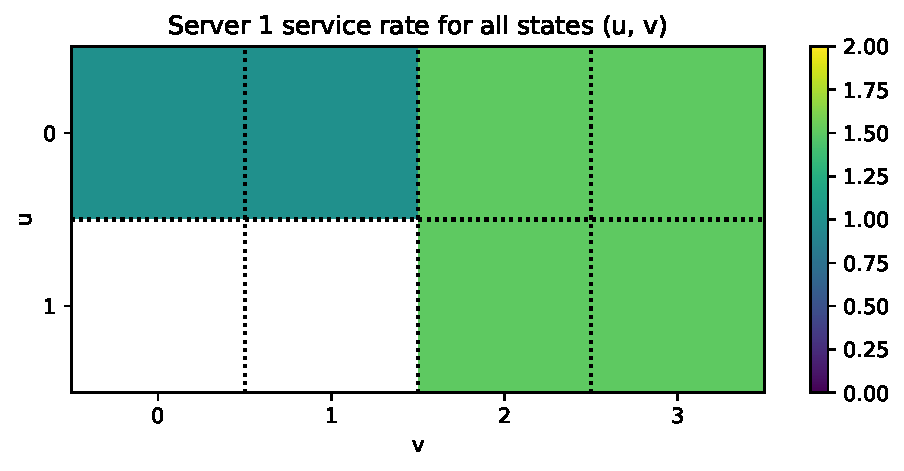
\includegraphics[width=0.45\textwidth]{chapters/06_agent_based_extension/Bin/reinforcement_learning_policy_example/server_1_1.pdf}
    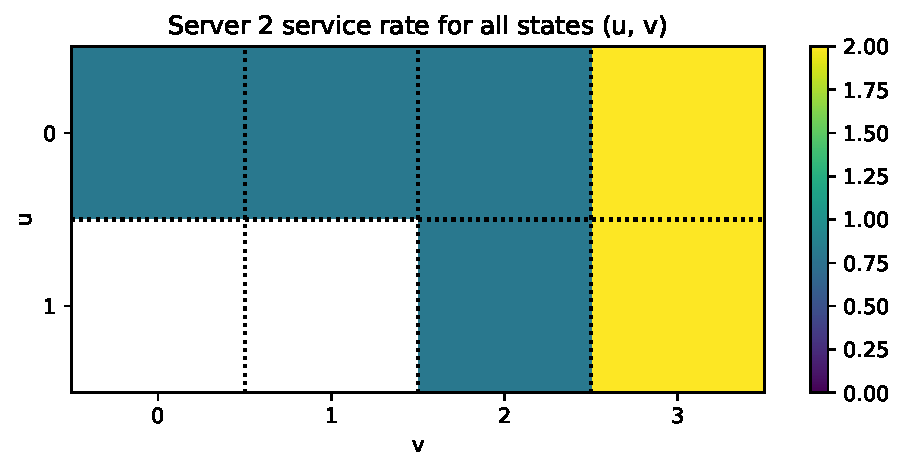
\includegraphics[width=0.45\textwidth]{chapters/06_agent_based_extension/Bin/reinforcement_learning_policy_example/server_2_1.pdf}
    \caption{Example policy for server \(1\) and server \(2\) at time step \(1\)}
    \label{fig:reinforcement_learning_policy_exmaple_1}
\end{figure}


\begin{figure}[H]
    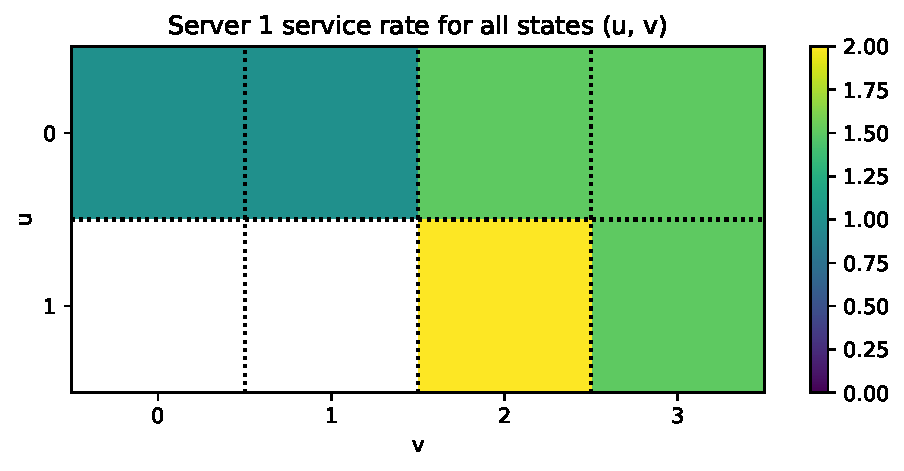
\includegraphics[width=0.45\textwidth]{chapters/06_agent_based_extension/Bin/reinforcement_learning_policy_example/server_1_2.pdf}
    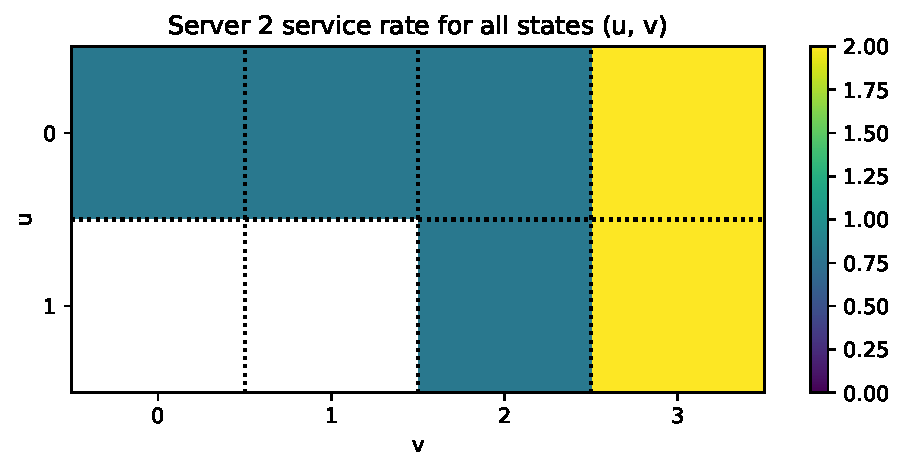
\includegraphics[width=0.45\textwidth]{chapters/06_agent_based_extension/Bin/reinforcement_learning_policy_example/server_2_2.pdf}
    \caption{Example policy for server \(1\) and server \(2\) at time step \(2\)}
    \label{fig:reinforcement_learning_policy_exmaple_2}
\end{figure}

\begin{figure}[H]
    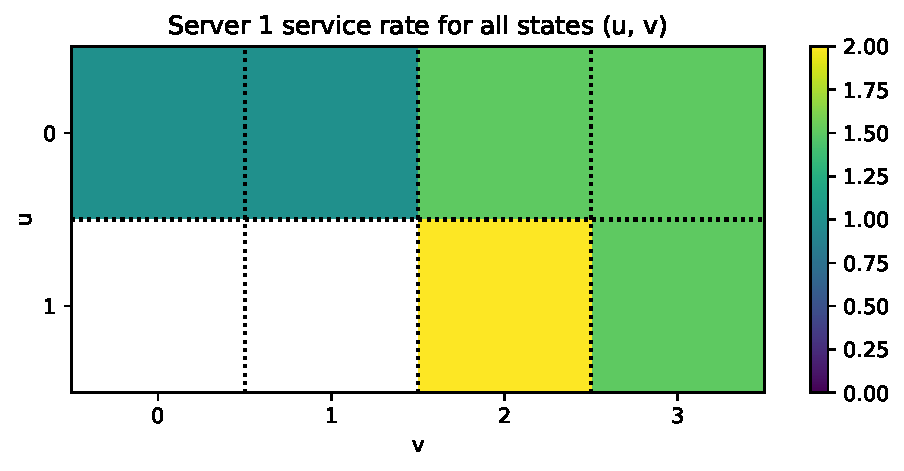
\includegraphics[width=0.45\textwidth]{chapters/06_agent_based_extension/Bin/reinforcement_learning_policy_example/server_1_3.pdf}
    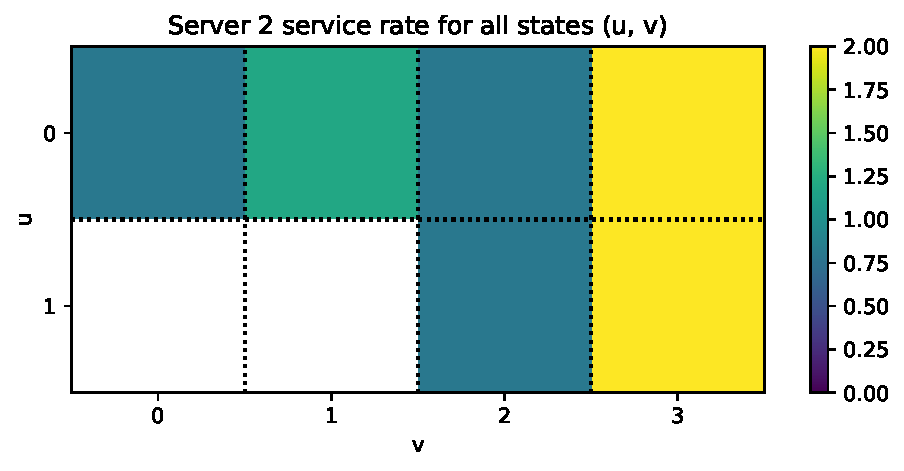
\includegraphics[width=0.45\textwidth]{chapters/06_agent_based_extension/Bin/reinforcement_learning_policy_example/server_2_3.pdf}
    \caption{Example policy for server \(1\) and server \(2\) at time step \(3\)}
    \label{fig:reinforcement_learning_policy_exmaple_3}
\end{figure}



\subsection{Numeric results}\label{sec:reiforcement_learning_numeric_results}

The reinforcement learning algorithm is implemented in python and the scripts
along with the generated data presented in this section have been archived and
can be found in~\cite{michalis_panayides_2023_7586860}.
Additional numerical experiments can also be found in
Appendix~\ref{appendix:reinforcement_learning}.

Consider a queueing system with the following parameters:

\begin{multicols}{4}
    \begin{itemize}
        \item \(\lambda_2 = 1\)
        \item \(\lambda_1 = 0.5 \)
        \item \(\mu = 0.7\)
        \item \(C = 4\)
        \item \(T = 7\)
        \item \(N = 10\)
        \item \(M = 7 \)
    \end{itemize}
\end{multicols}

Note that for the initial policy, the service rates of the \(4\) servers are
set to \(\mu = 0.7\) for all servers and all states.
In addition, the \(4\) servers are set to be of the same expertise level as
described in Section~\ref{sec:agent_based_case_study}.
That is, server \(1\) is an experienced server, server \(2\) and server
\(3\) are moderate servers and server \(4\) is an intern.
That means that when server \(1\) is not busy they will always receive the
incoming individual, otherwise either server \(2\) or server \(3\) will
receive that individual with an equal probability.
Finally, server \(4\) may serve an individual only when every other server is
busy.

The remaining of this section focuses on the results of the reinforcement
learning algorithm from using utility functions \(U_k^{(3)}\) and
\(U_k^{(7)}\) with different values of \(e\).
The two utility functions are chosen because they were considered to be the
most realistic ones.
In addition utility function \(U_k^{(7)}\) is used to express the effect of
having to balance the server's best interest with the system's best interest.
It is assumed that a server would like the proportion of individuals served
to be as high as possible, while also maximising their own idle time.
This is what utility function \(U_k^{(7)}\) aims to capture.

\subsubsection{Utility function 3 \((U_k^{(3)})\) with \(e = 0.1\)}
\label{sec:utility_3_results}

Consider utility function 3 defined in~\eqref{eq:utility_3} where
\(U_k^{(3)} = e \, \bar{m}^{(k)} + (1 - e) \, (R - B^{(k)})\).
Thus a server's utility corresponds to the weighted average of the server's
service time and their idle time.
This means that in order for servers to increase their utility they either
need to work faster or increase the amount of time they are idle.
Figure~\ref{fig:RL_utility3_1_e01} shows the utilities and mean service rate
of servers from the reinforcement learning run using utility function
\(U_k^{(3)}\) with \(e = 0.1\) and \(100,\!000\) time steps.

\begin{figure}[H]
    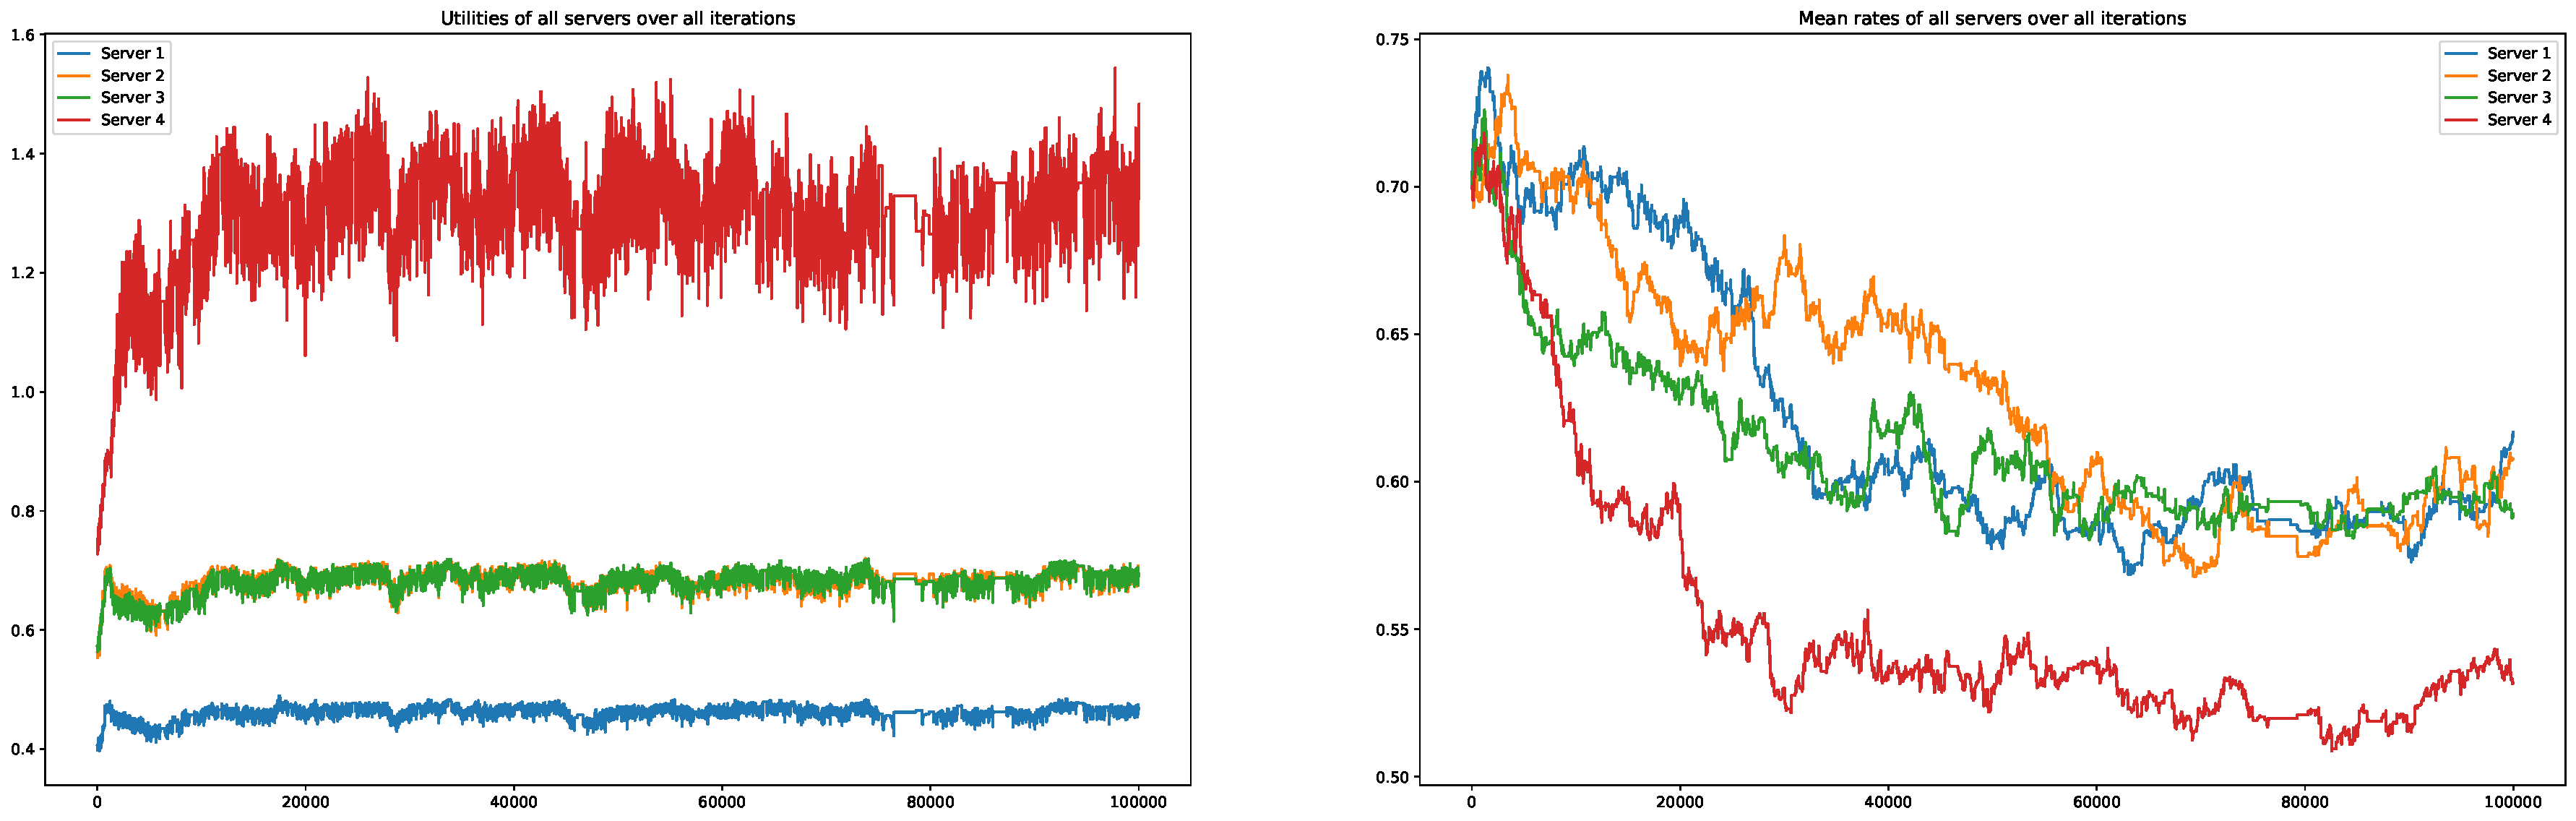
\includegraphics[width=\textwidth]{chapters/06_agent_based_extension/Bin/reinforcement_learning_results/utility_3/u3_1_e01.pdf}
    \caption{Utilities (left) and mean service rate (right) of servers from the
    reinforcement learning run using utility function \(U_k^{(3)}\) with
    \(e = 0.1\) and \(100,\!000\) time steps}
    \label{fig:RL_utility3_1_e01}
\end{figure}

It can be seen from Figure~\ref{fig:RL_utility3_1_e01} that the utility of
server \(1\) (that has the highest priority on incoming individuals) is the
lowest, while server \(4\) (that has the lowest priority on incoming)
individuals has the highest utility.
In addition, the mean service rate of server \(4\) is the lowest while servers
\(1\), \(2\) and \(3\) have similar mean service rates.
All servers managed to increase their utility by reducing their mean service
rate (i.e. working faster).
Figure~\ref{fig:RL_utility3_2_e01} shows the same example as above but with
\(500,\!000\) time steps.

\begin{figure}[H]
    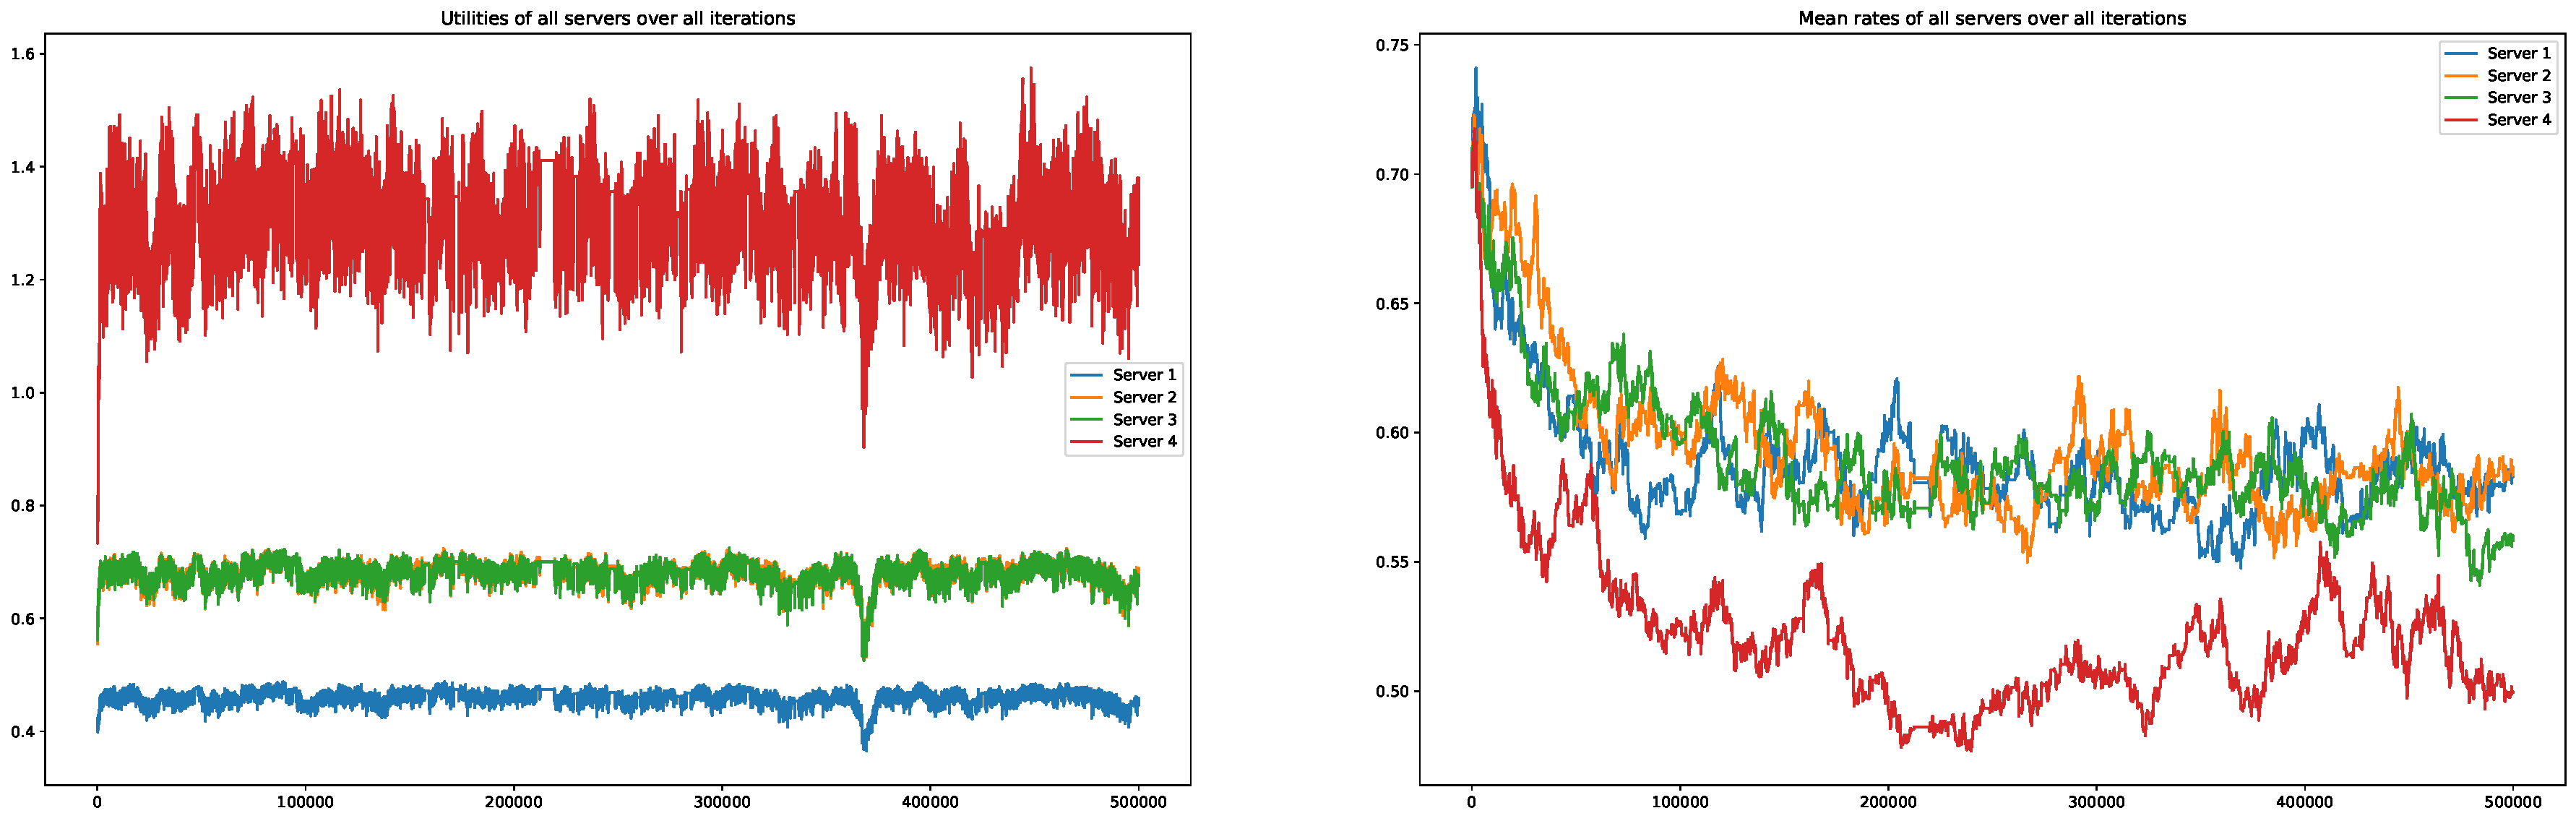
\includegraphics[width=\textwidth]{chapters/06_agent_based_extension/Bin/reinforcement_learning_results/utility_3/u3_2_e01.pdf}
    \caption{Utilities (left) and mean service rate (right) of servers from the
    reinforcement learning run using utility function \(U_k^{(3)}\) with
    \(e = 0.1\) and \(500,\!000\) time steps}
    \label{fig:RL_utility3_2_e01}
\end{figure}

Running the algorithm again for a longer runtime of \(500,\!000\) time steps
does not change the results significantly.
The same observations can be made for both figures.



\subsubsection{Utility function 7 \((U_k^{(7)})\) with \(e = 0.1\)}
\label{sec:utility_7_01_results}

Consider the plot of the mean rates of
Figures~\ref{fig:RL_utility3_1_e01}~and~\ref{fig:RL_utility3_2_e01}
(rightmost graph).
The service rate of each server consists of a different service rate for each
state \((u, v)\) of the system.
The way the reinforcement learning algorithm is constructed, the service rate
of each server is updated at each time step based on the visited states of the
system.
This means that it doesn't make sense to calculate the mean service rate from
all states of the system.
In this subsection, the weighted mean service rate is used instead, where
the weight of each state is the probability of visiting that state.
The weighted mean service rate of server \(k\) is defined as:

\begin{equation}
    \hat{\mu}^{(k)} = \sum_{(u, v) \in \mathcal{S}} \,
    \pi(u, v) \, \mu_{k, (u, v)}
\end{equation}

Consider the same example as in the previous subsection but with utility
function 7 defined in~\eqref{eq:utility_7} where
\(U_k^{(7)} = e \, \frac{I_s}{I} + (1 - e) \, \frac{R - B^{(k)}}{R}\) and
\(e = 0.1\).
Note that given the nature of this utility function the utilities of the agents
can now only be within the range \([0, 1]\).

\begin{figure}[H]
    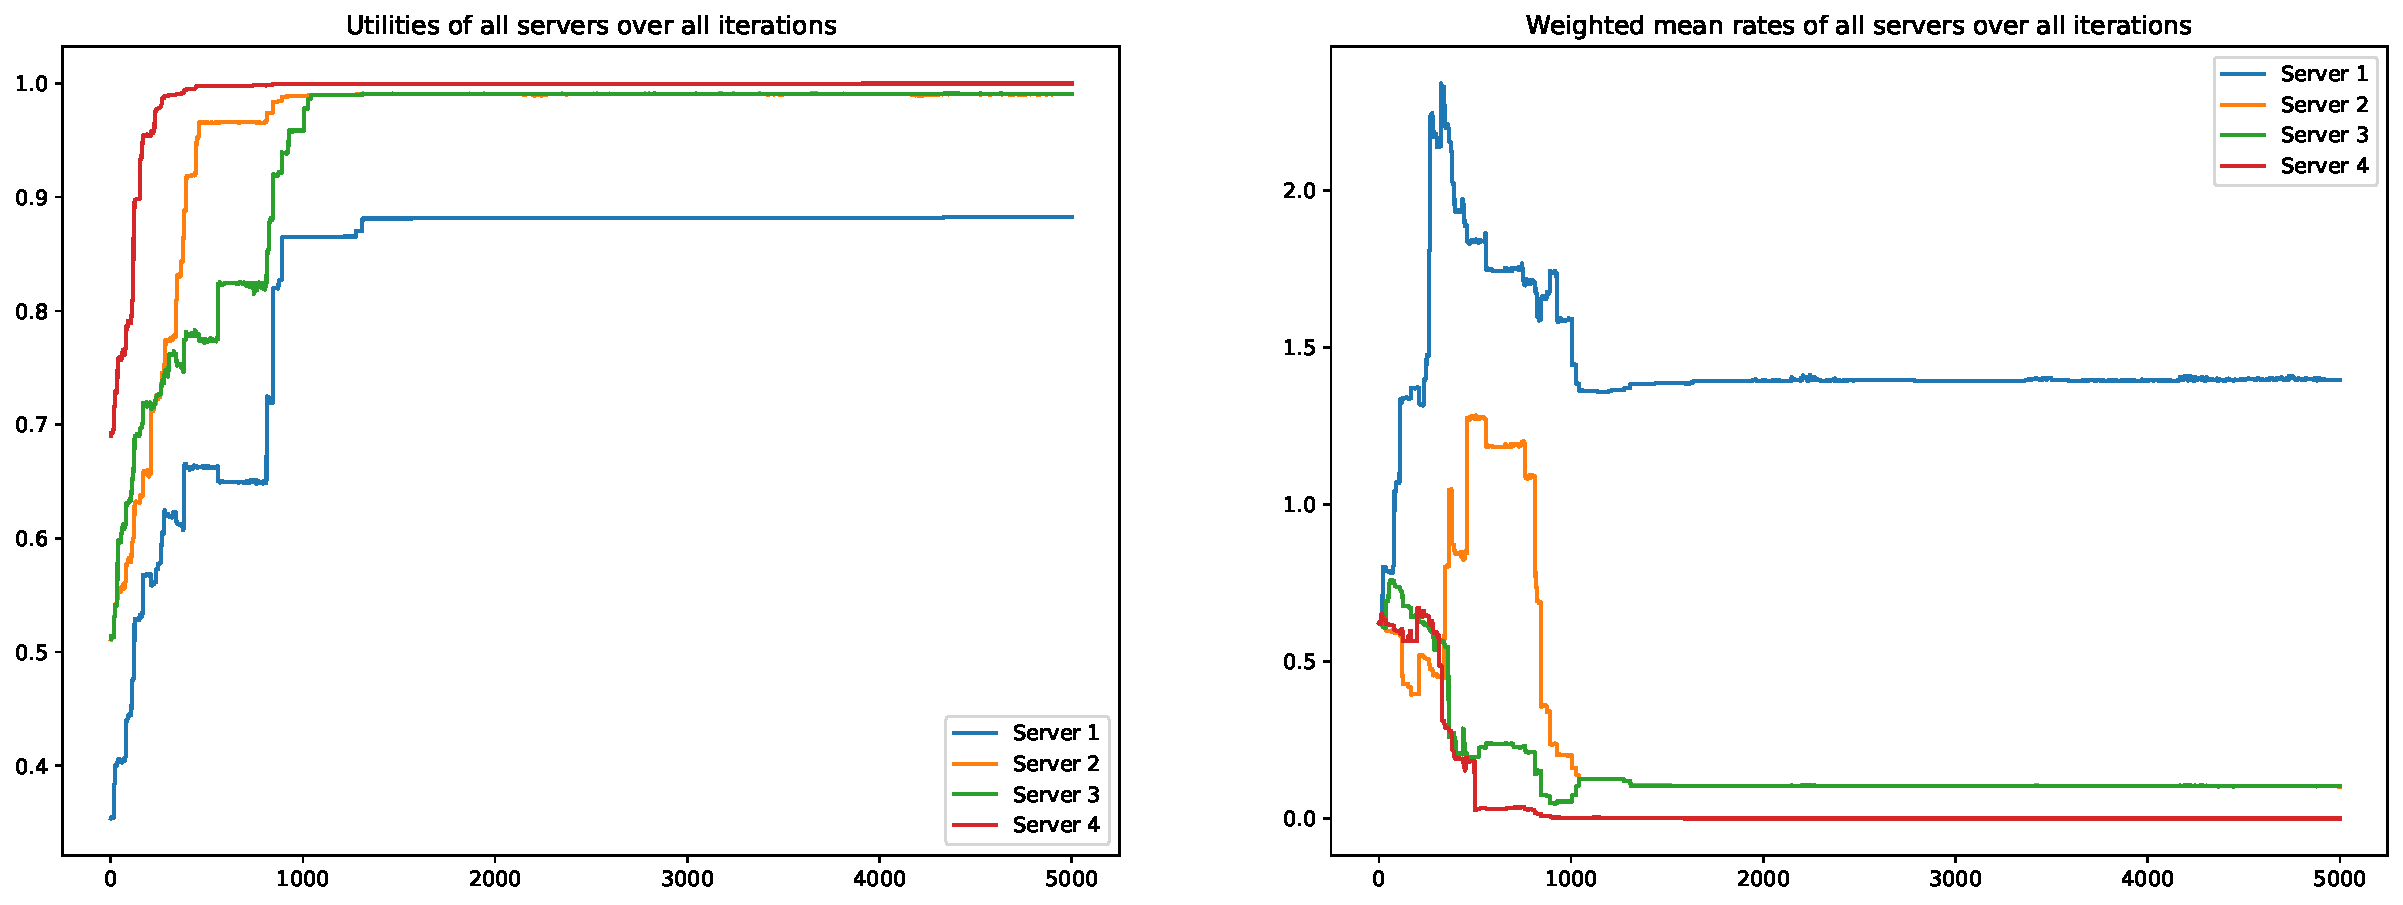
\includegraphics[width=\textwidth]{chapters/06_agent_based_extension/Bin/reinforcement_learning_results/utility_7/u7_4_e01.pdf}
    \caption{Utilities (left) and weighted mean service rate (right) of servers
    from the reinforcement learning run using utility function \(U_k^{(7)}\)
    with \(e = 0.1\).}
    \label{fig:RL_utility7_4_e01}
\end{figure}

Figure~\ref{fig:RL_utility7_4_e01} shows the utilities and weighted mean
service rate of servers from the reinforcement learning run using utility
function \(U_k^{(7)}\).
It can be seen from Figure~\ref{fig:RL_utility7_4_e01} that the utilities
follow a similar pattern to the ones from Section~\ref{sec:utility_3_results}.
That is, the utility of server \(1\) is the lowest while the utility of server
\(4\) is the highest, leaving servers \(2\) and \(3\) with similar utilities
in between.
In terms of the weighted mean service rate, servers \(2\), \(3\) and \(4\)
managed to reduce their service rate while server \(1\) had to increase its
service rate in order to maximise its utility.

What happens if the initial service rate of all servers is changed?
Would the servers manage to arrive to the same policies and same utilities?
Figure~\ref{fig:RL_utility7_4_e01_initial_02} shows the utilities and weighted
mean service rates of servers from the reinforcement learning run using utility
function \(U_k^{(7)}\) with \(e = 0.1\) and an initial service rate of
\(0.2\) for all servers.

\begin{figure}[H]
    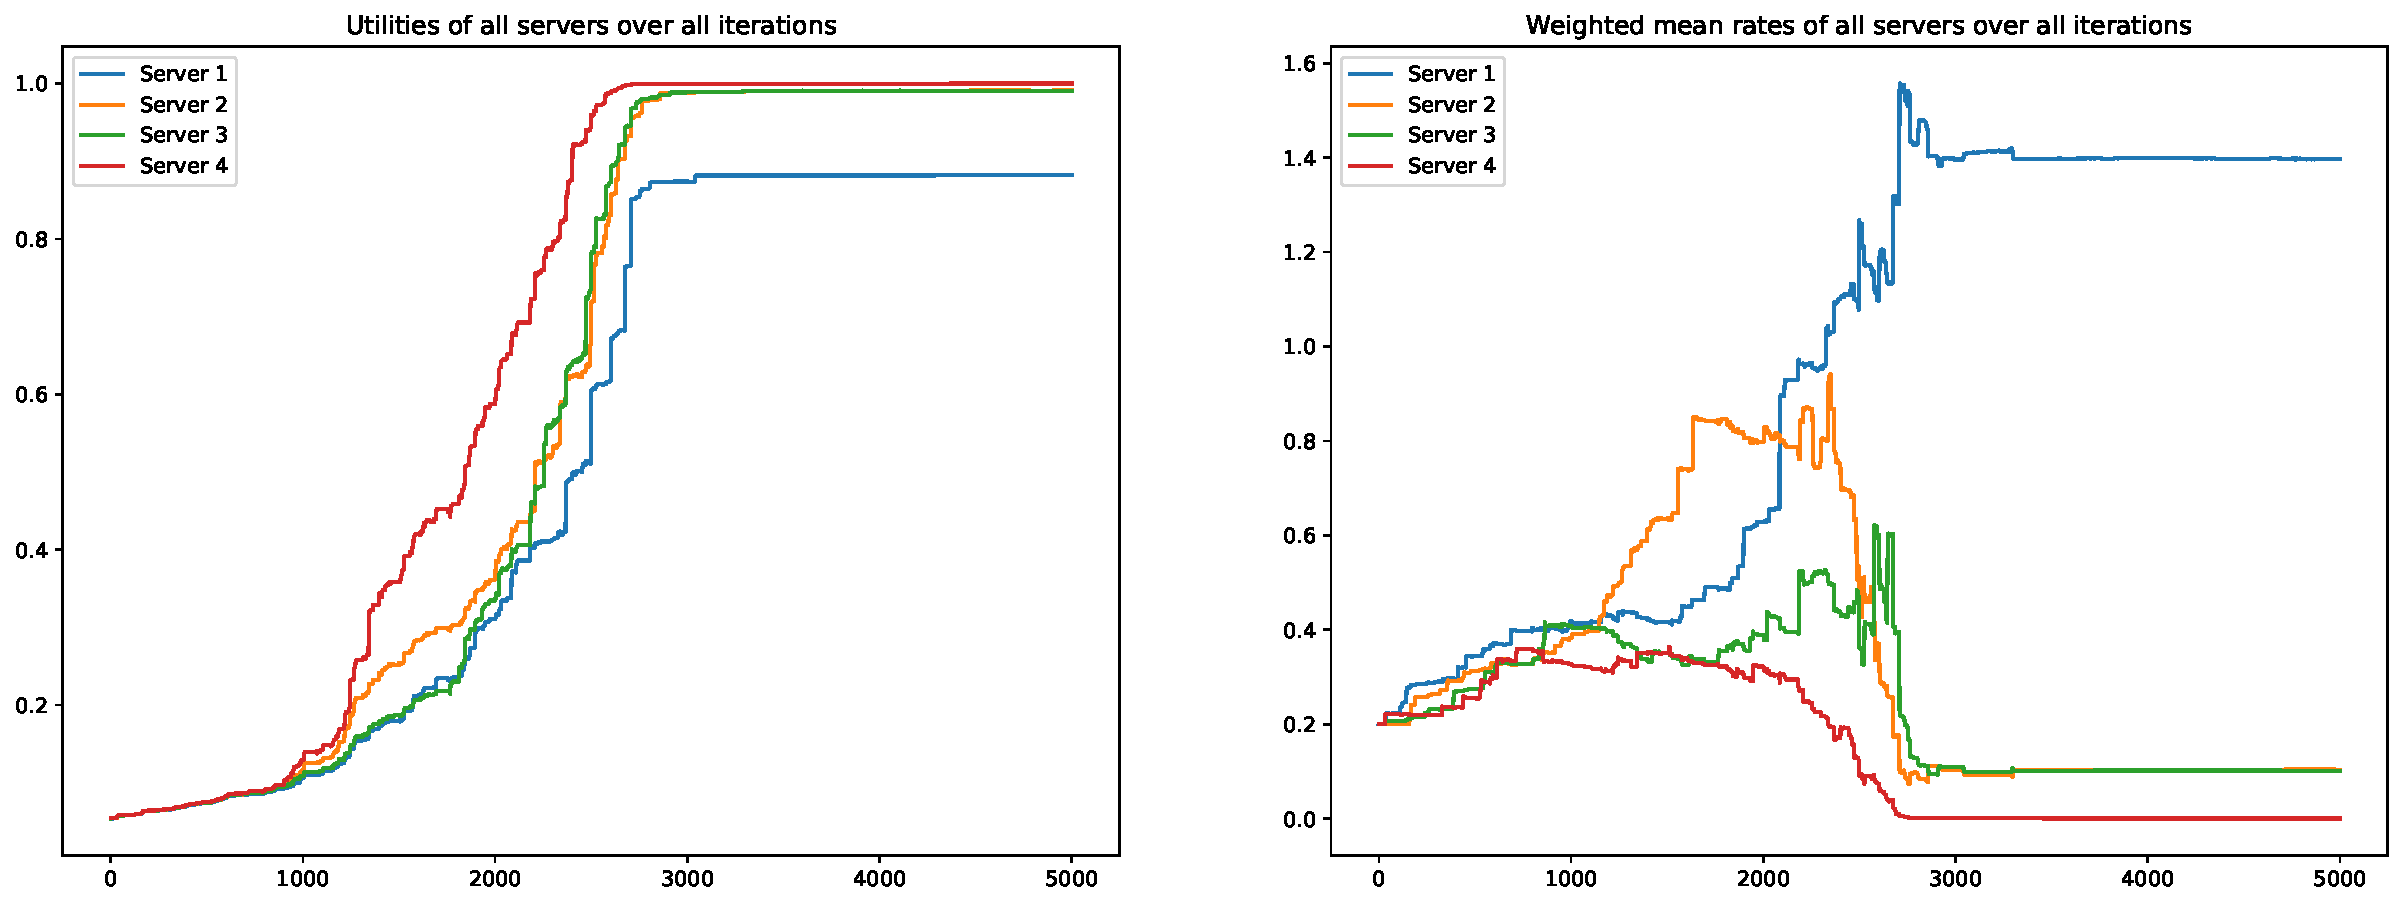
\includegraphics[width=\textwidth]{chapters/06_agent_based_extension/Bin/reinforcement_learning_results/utility_7/u7_4_e01_initial_02.pdf}
    \caption{Utilities (left) and weighted mean service rate (right) of servers
    from the reinforcement learning run using utility function \(U_k^{(7)}\)
    with \(e = 0.1\) and an initial service rate of \(0.2\) for all servers.}
    \label{fig:RL_utility7_4_e01_initial_02}
\end{figure}

Figure~\ref{fig:RL_utility7_4_e01_initial_02} shows that, even though it takes
longer to stabilise, the reinforcement learning algorithm is able to find the
same utilities as before.
In addition, it can be seen from the weighted mean service rates that servers
have also managed to find the same policies as before.
Note that more exploration is needed from the agents in order to reach the
same policies as before.

Now, consider the scenario where the initial service rate of all servers is
increased.
Figure~\ref{fig:RL_utility7_4_e01_initial_15} shows the utilities and weighted
mean service rates of servers from the reinforcement learning run using utility
function \(U_k^{(7)}\) with \(e = 0.1\) and an initial service rate of
\(1.5\) for all servers.

\begin{figure}[H]
    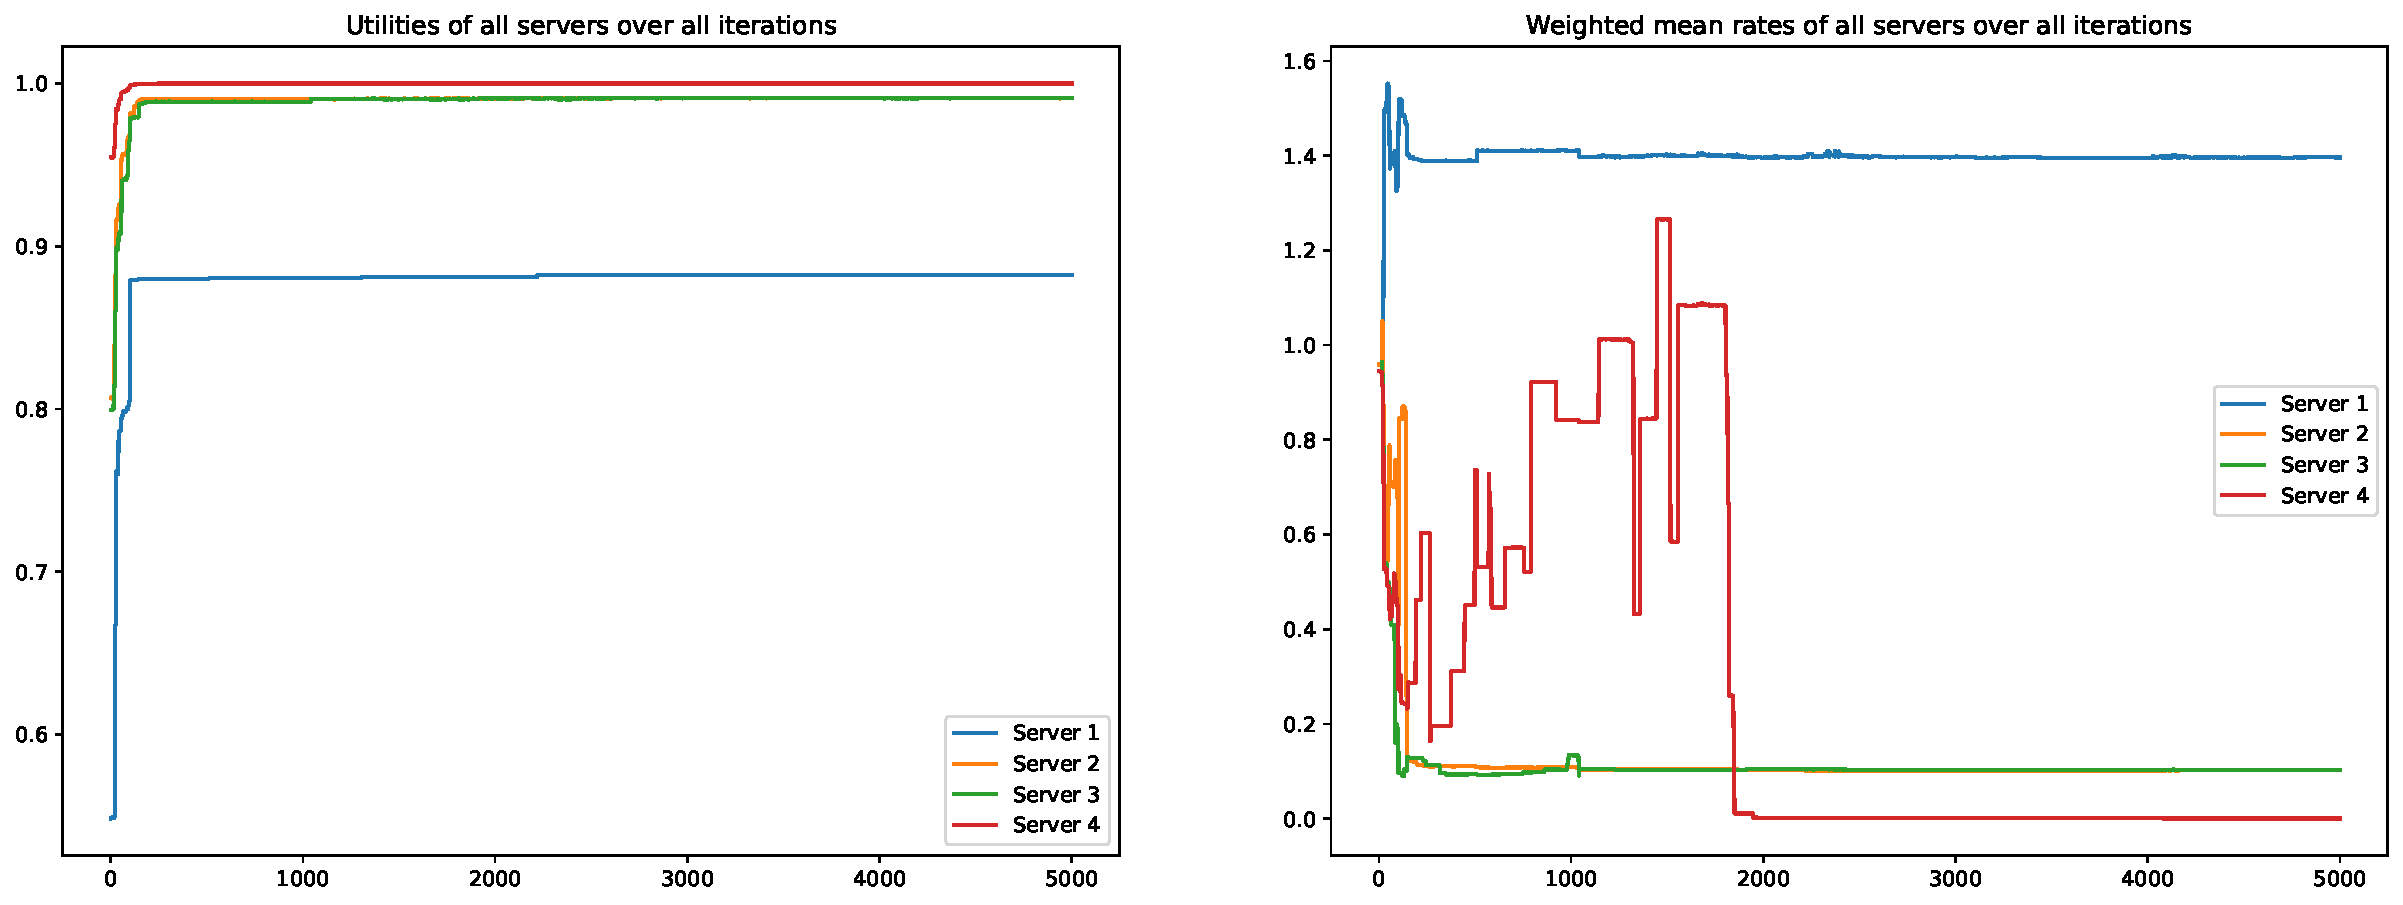
\includegraphics[width=\textwidth]{chapters/06_agent_based_extension/Bin/reinforcement_learning_results/utility_7/u7_4_e01_initial_15.pdf}
    \caption{Utilities (left) and weighted mean service rate (right) of servers
    from the reinforcement learning run using utility function \(U_k^{(7)}\)
    with \(e = 0.1\) and an initial service rate of \(1.5\) for all servers.}
    \label{fig:RL_utility7_4_e01_initial_15}
\end{figure}





\subsubsection{Utility function 7 \((U_k^{(7)})\) with e = 0.5}
\label{sec:utility_7_05_results}

This subsection considers the same parameters and utility function as in
Section~\ref{sec:utility_7_01_results} but with a different value for
parameter \(e\).
Figure~\ref{fig:RL_utility7_4_e05} shows the utilities and weighted mean
service rates of servers from the reinforcement learning run using utility
function \(U_k^{(7)}\) with \(e = 0.5\).

\begin{figure}[H]
    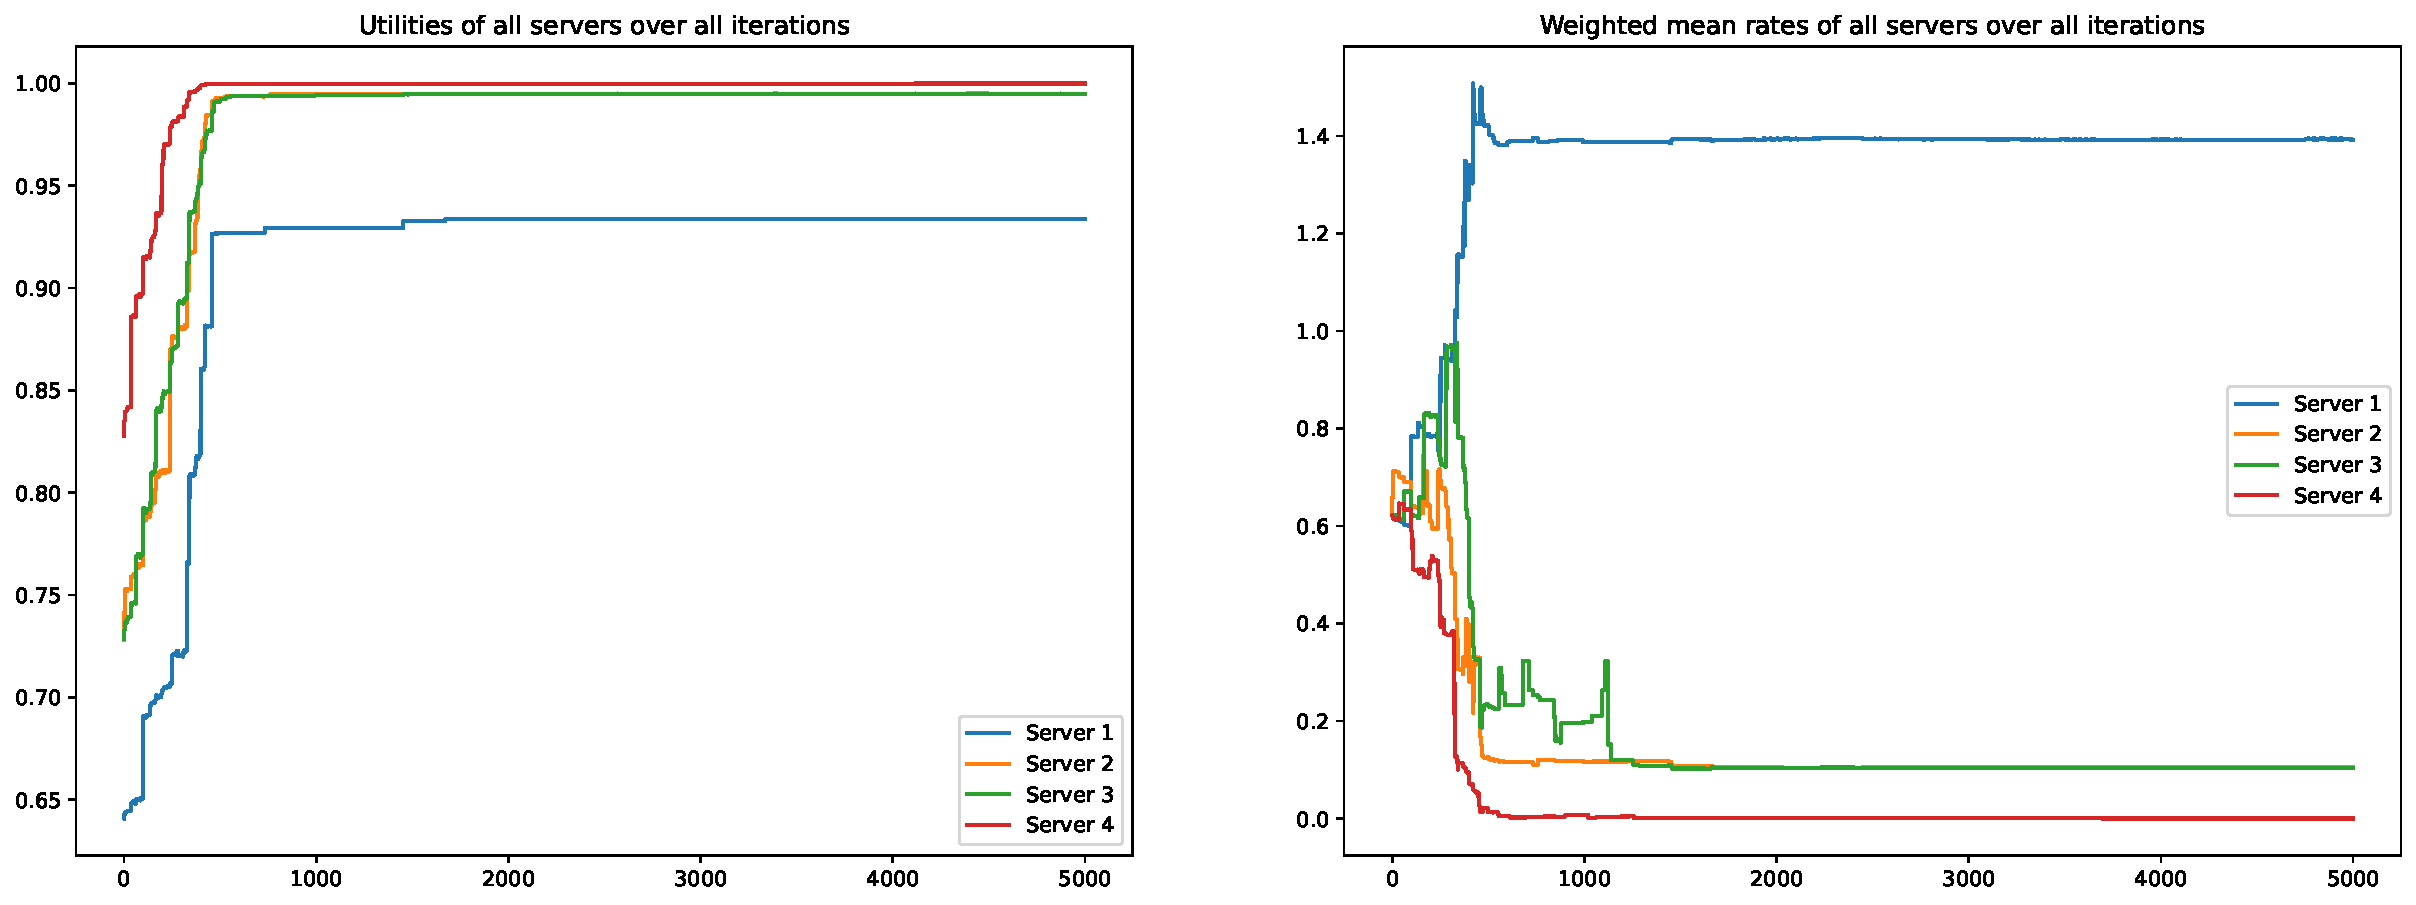
\includegraphics[width=\textwidth]{chapters/06_agent_based_extension/Bin/reinforcement_learning_results/utility_7/u7_4_e05.pdf}
    \caption{Utilities (left) and weighted mean service rate (right) of servers
    from the reinforcement learning run using utility function \(U_k^{(7)}\)
    with \(e = 0.5\).}
    \label{fig:RL_utility7_4_e05}
\end{figure}

A similar pattern to the one in Figure~\ref{fig:RL_utility7_4_e01} can be seen
from Figure~\ref{fig:RL_utility7_4_e05}.
The policies found by the agents at the end of the run are similar to the ones
found when using \(e = 0.1\).
The only difference is that the utilities are slightly higher when using
\(e = 0.5\).

Consider the scenario where the arrival rates of the two servers are increased.
Figure~\ref{fig:RL_utility7_4_e05_Lambda_45} shows the utilities and weighted
mean service rates of servers when increasing arrival rates of
\(\lambda_1 = 2\) and \(\lambda_2 = 2.5\).

\begin{figure}[H]
    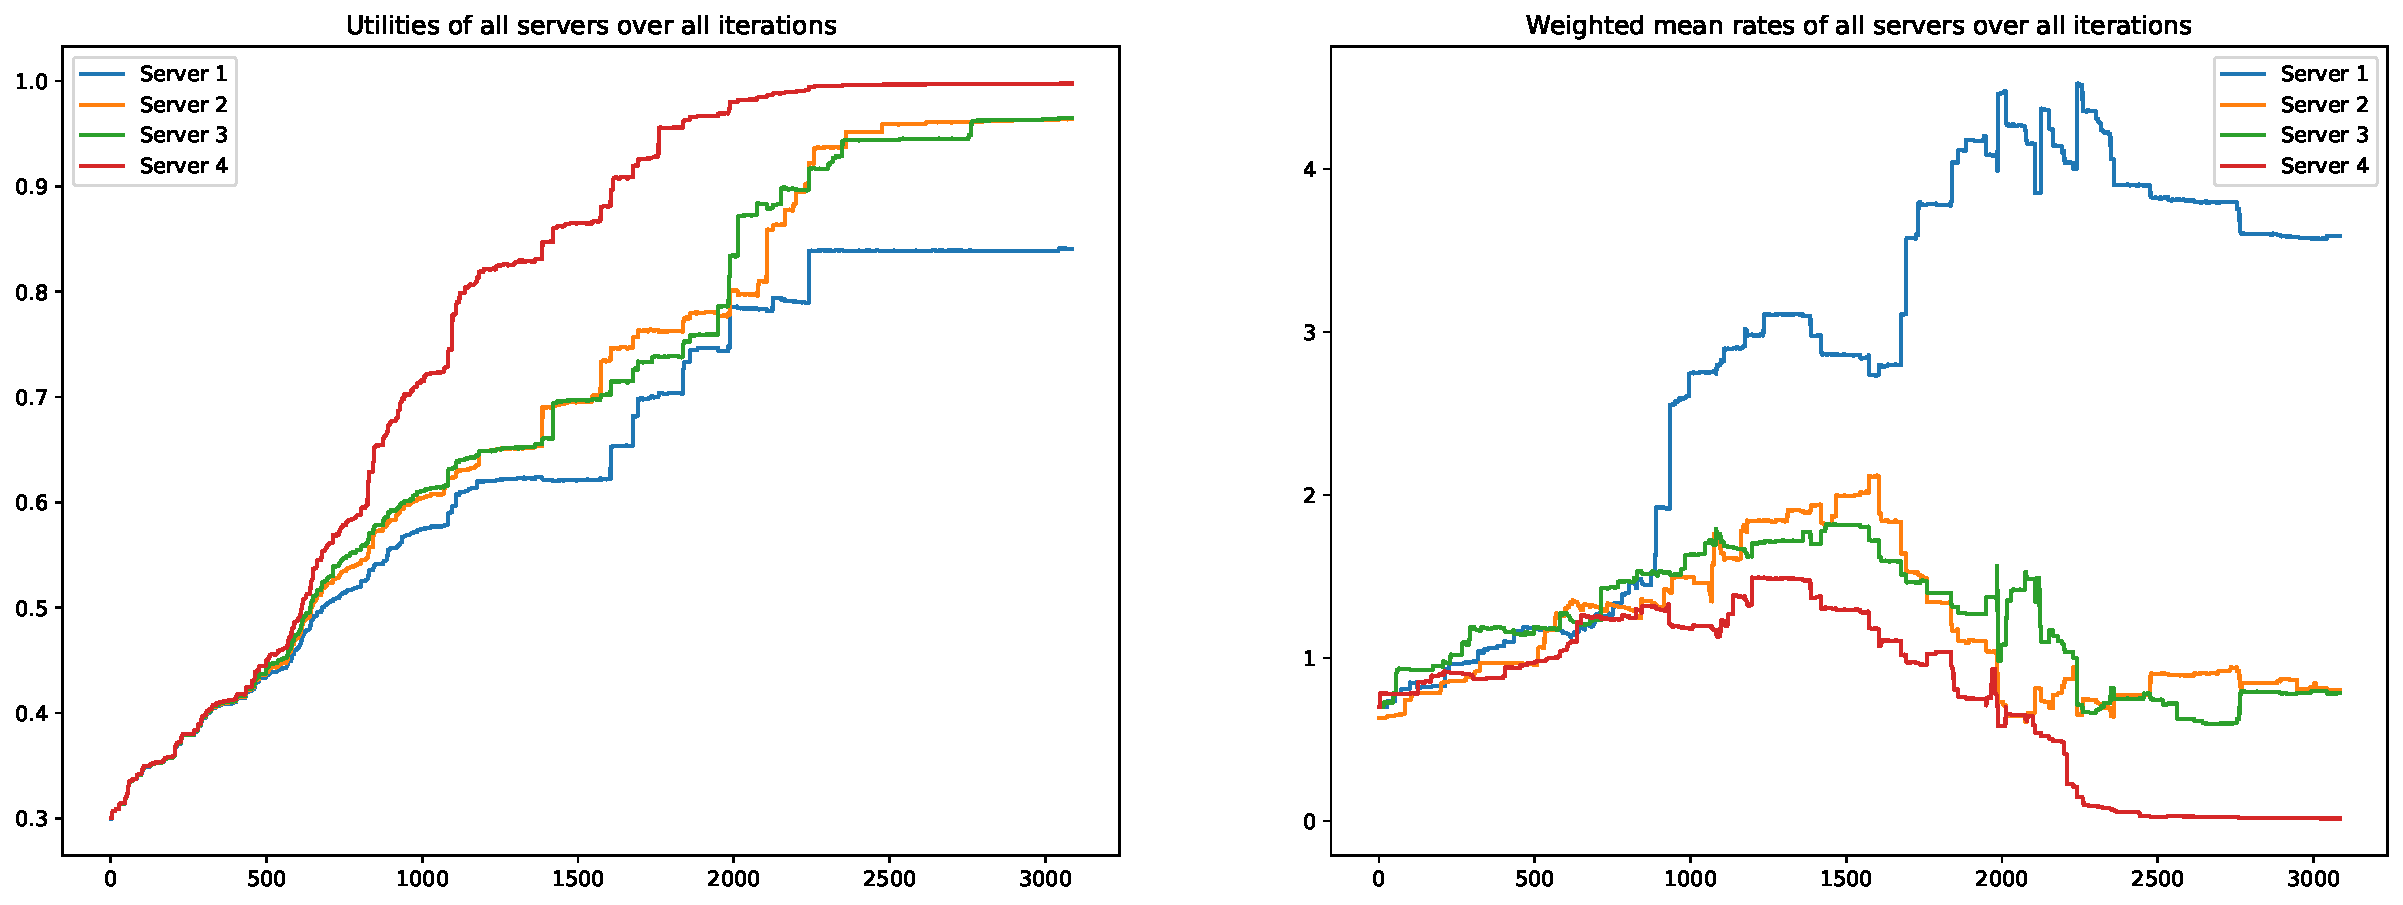
\includegraphics[width=\textwidth]{chapters/06_agent_based_extension/Bin/reinforcement_learning_results/utility_7/u7_4_e05_Lambda_45.pdf}
    \caption{Utilities (left) and weighted mean service rate (right) of servers
    from the reinforcement learning run using utility function \(U_k^{(7)}\)
    with \(e = 0.5\) and increased arrival rates of \(\lambda_1 = 2\) and
    \(\lambda_2 = 2.5\).}
    \label{fig:RL_utility7_4_e05_Lambda_45}
\end{figure}


\subsubsection{Utility function 7 \((U_k^{(7)})\) with no upper bounds}
\label{sec:utility_7_no_upper_bound_results}

Numeric results of Sections~\ref{sec:utility_3_results},
\ref{sec:utility_7_01_results} and \ref{sec:utility_7_05_results} use an upper
bound for the service rate of servers.
In other words, the service rate of servers is bounded by a specific value
so that the agents don't end up with a service rate of a really high
unrealistic value.
An example of the reinforcement learning run using utility function
\(U_k^{(7)}\) with \(e = 0.5\) and no upper bound on the service rate is
shown in Figure~\ref{fig:RL_utility7_5_no_max_e05}.

\begin{figure}[H]
    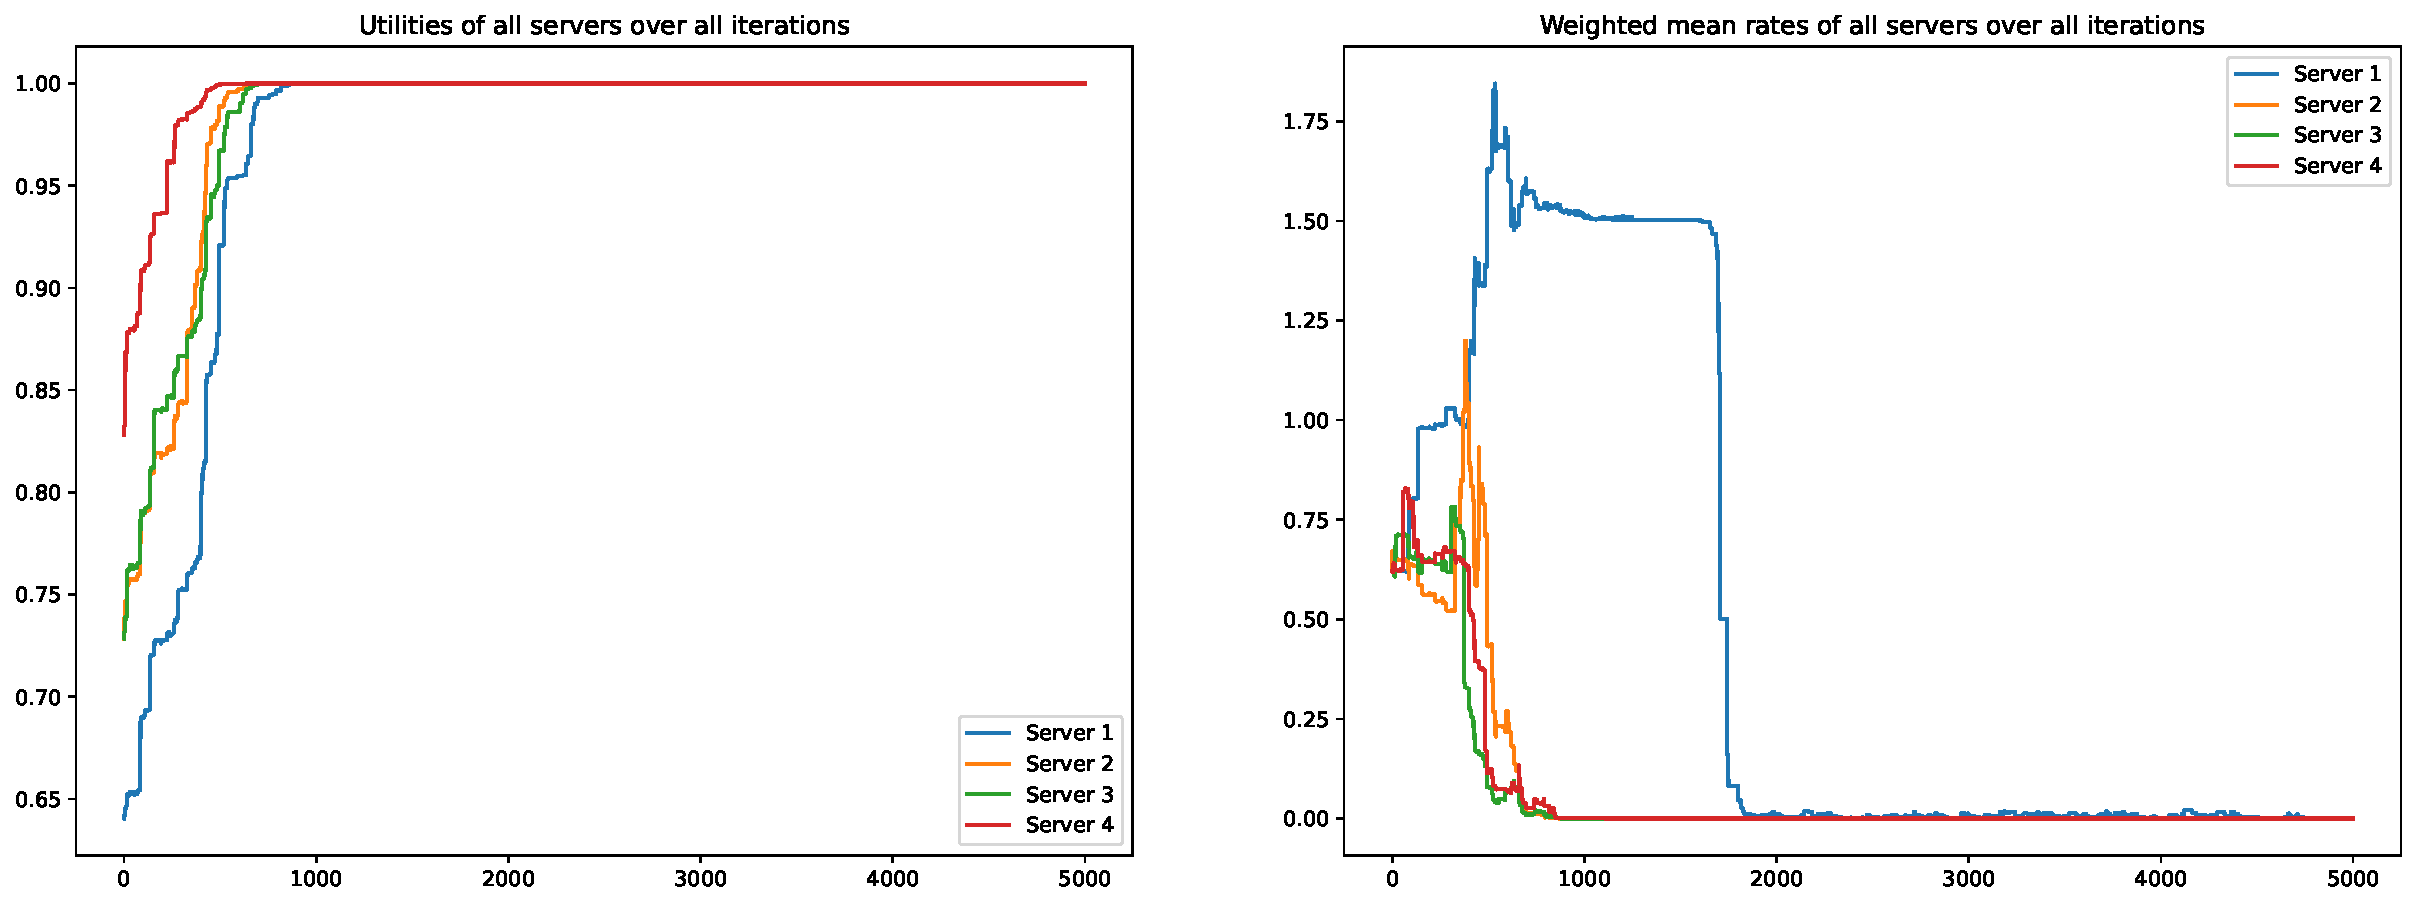
\includegraphics[width=\textwidth]{chapters/06_agent_based_extension/Bin/reinforcement_learning_results/utility_7/u7_5_no_max_e05.pdf}
    \caption{Utilities (left) and weighted mean service rate (right) of servers
    from the reinforcement learning run using utility function \(U_k^{(7)}\)
    with \(e = 0.5\) and no upper bound on the service rate.}
    \label{fig:RL_utility7_5_no_max_e05}
\end{figure}

It can be seen from Figure~\ref{fig:RL_utility7_5_no_max_e05} that the
reinforcement learning algorithm ends up with a weighted mean service rate of
servers of \(0\) while getting all their utilities to the maximum value of
\(1\).
The question to be asked is how something like this is possible.
The answer is that since the service rate of servers is not bounded, server
\(1\) ends up having a ridiculously high service rate.
The service rates of the remaining servers don't matter since every individual
that arrives, is served by server \(1\) almost instantly and leaves the system
immediately.
This results in the state probabilities being \(0\) in every state except state
\(0,0\).
In fact, only states \(0,0\) and \(0,1\) are visited in the system, where
\(0,1\) is visited for a short time because of how fast server \(1\) is
serving individuals.


\scriptsize
\begin{equation}\label{eq:no_upper_bound_states_example}
\begin{bmatrix}
    1.0 & 2.44\times10^{-19} & \text{NaN} & \text{NaN} & \text{NaN} & \text{NaN}
    & \text{NaN} & \text{NaN} & \text{NaN} & \text{NaN} & \text{NaN} \\
    \text{NaN} & \text{NaN} & \text{NaN} & \text{NaN} & \text{NaN} & \text{NaN}
    & \text{NaN} & \text{NaN} & \text{NaN} & \text{NaN} & \text{NaN} \\
    \text{NaN} & \text{NaN} & \text{NaN} & \text{NaN} & \text{NaN} & \text{NaN}
    & \text{NaN} & \text{NaN} & \text{NaN} & \text{NaN} & \text{NaN} \\
    \text{NaN} & \text{NaN} & \text{NaN} & \text{NaN} & \text{NaN} & \text{NaN}
    & \text{NaN} & \text{NaN} & \text{NaN} & \text{NaN} & \text{NaN} \\
    \text{NaN} & \text{NaN} & \text{NaN} & \text{NaN} & \text{NaN} & \text{NaN}
    & \text{NaN} & \text{NaN} & \text{NaN} & \text{NaN} & \text{NaN} \\
    \text{NaN} & \text{NaN} & \text{NaN} & \text{NaN} & \text{NaN} & \text{NaN}
    & \text{NaN} & \text{NaN} & \text{NaN} & \text{NaN} & \text{NaN} \\
    \text{NaN} & \text{NaN} & \text{NaN} & \text{NaN} & \text{NaN} & \text{NaN}
    & \text{NaN} & \text{NaN} & \text{NaN} & \text{NaN} & \text{NaN} \\
    \text{NaN} & \text{NaN} & \text{NaN} & \text{NaN} & \text{NaN} & \text{NaN}
    & \text{NaN} & \text{NaN} & \text{NaN} & \text{NaN} & \text{NaN} \\
\end{bmatrix}
\end{equation}

\begin{equation}\label{eq:no_upper_bound_rates_example}
\begin{bmatrix}
    0 & 4\times10^{15} & 9.4 & 0.5 & 2.1 & 1.8 & 0.8 & 0.4 & 0.7 & 0.7 & 0.7 \\
    \text{NaN} & \text{NaN} & \text{NaN} & \text{NaN} & \text{NaN} & \text{NaN}
    & \text{NaN} & 0.7 & 1.9 & 0.08 & 0.7 \\
    \text{NaN} & \text{NaN} & \text{NaN} & \text{NaN} & \text{NaN} & \text{NaN}
    & \text{NaN} & 1.6 & 0.7 & 0.1 & 0.7 \\
    \text{NaN} & \text{NaN} & \text{NaN} & \text{NaN} & \text{NaN} & \text{NaN}
    & \text{NaN} & 1.3 & 0.7 & 0.7 & 0.7 \\
    \text{NaN} & \text{NaN} & \text{NaN} & \text{NaN} & \text{NaN} & \text{NaN}
    & \text{NaN} & 0.7 & 0.2 & 0.7 & 0.7 \\
    \text{NaN} & \text{NaN} & \text{NaN} & \text{NaN} & \text{NaN} & \text{NaN}
    & \text{NaN} & 0.7 & 0.7 & 0.7 & 0.7 \\
    \text{NaN} & \text{NaN} & \text{NaN} & \text{NaN} & \text{NaN} & \text{NaN}
    & \text{NaN} & 0.7 & 0.7 & 0.7 & 0.7 \\
    \text{NaN} & \text{NaN} & \text{NaN} & \text{NaN} & \text{NaN} & \text{NaN}
    & \text{NaN} & 0.7 & 0.7 & 0.7 & 0.7 \\
\end{bmatrix}
\end{equation}
\normalsize

Equation~\eqref{eq:no_upper_bound_states_example} shows the state probabilities
of the system and equation~\eqref{eq:no_upper_bound_rates_example} shows the
service rates of server \(1\).
The service rates of the remaining servers are not shown since they are not
relevant.
Note that the missing values in
equation~\eqref{eq:no_upper_bound_states_example} indicate that not only the
state probabilities are \(0\) for these states, but can't even be visited by
the system.
With a service rate of \(4\times10^{15}\) for server \(1\), state
probability \(2.44\times10^{-19}\) for state \(0,1\) and state probability
\(1.0\) for state \(0,0\), the weighted mean service rate of server \(1\) is:

\begin{equation}\label{eq:no_upper_bound_mean_rate_example}
    0\times2.44\times10^{-19} + 4\times10^{15}\times1.0 \approx 0.001
\end{equation}
 
That is the reason why an upper bound on the service rates is needed.
Without an upper bound, servers could choose an extremely high service rate and
thus making the system reach unreachable scenarios.

\subsubsection{Changing arrival rates during the run}
\label{subsubsec:reinforcement_learning_special_case}

Consider once again the same parameters and utility function as in
Section~\ref{sec:utility_7_05_results}.
That is a using a utility function \(U_k^{(7)}\) with \(e = 0.5\) and arrival
rates of \(\lambda_1 = 0.5\) and \(\lambda_2 = 1\).
In this subsection the reinforcement learning algorithm is run with the same
parameters, but the arrival rates are changed during the run.
The total runtime of the reinforcement learning algorithm is 5000 time steps.
The arrival rates are set to \(\lambda_1 = 0.5\) and \(\lambda_2 = 1\) for the
first \(2000\) time steps.
Then the arrival rates are increased to \(\lambda_1 = 3\) and
\(\lambda_2 = 3.5\) for time steps \(2000\) to \(4000\) and then the arrival
rates are decreased back to \(\lambda_1 = 0.5\) and \(\lambda_2 = 1\) for the
last \(1000\) time steps.

\begin{figure}[H]
    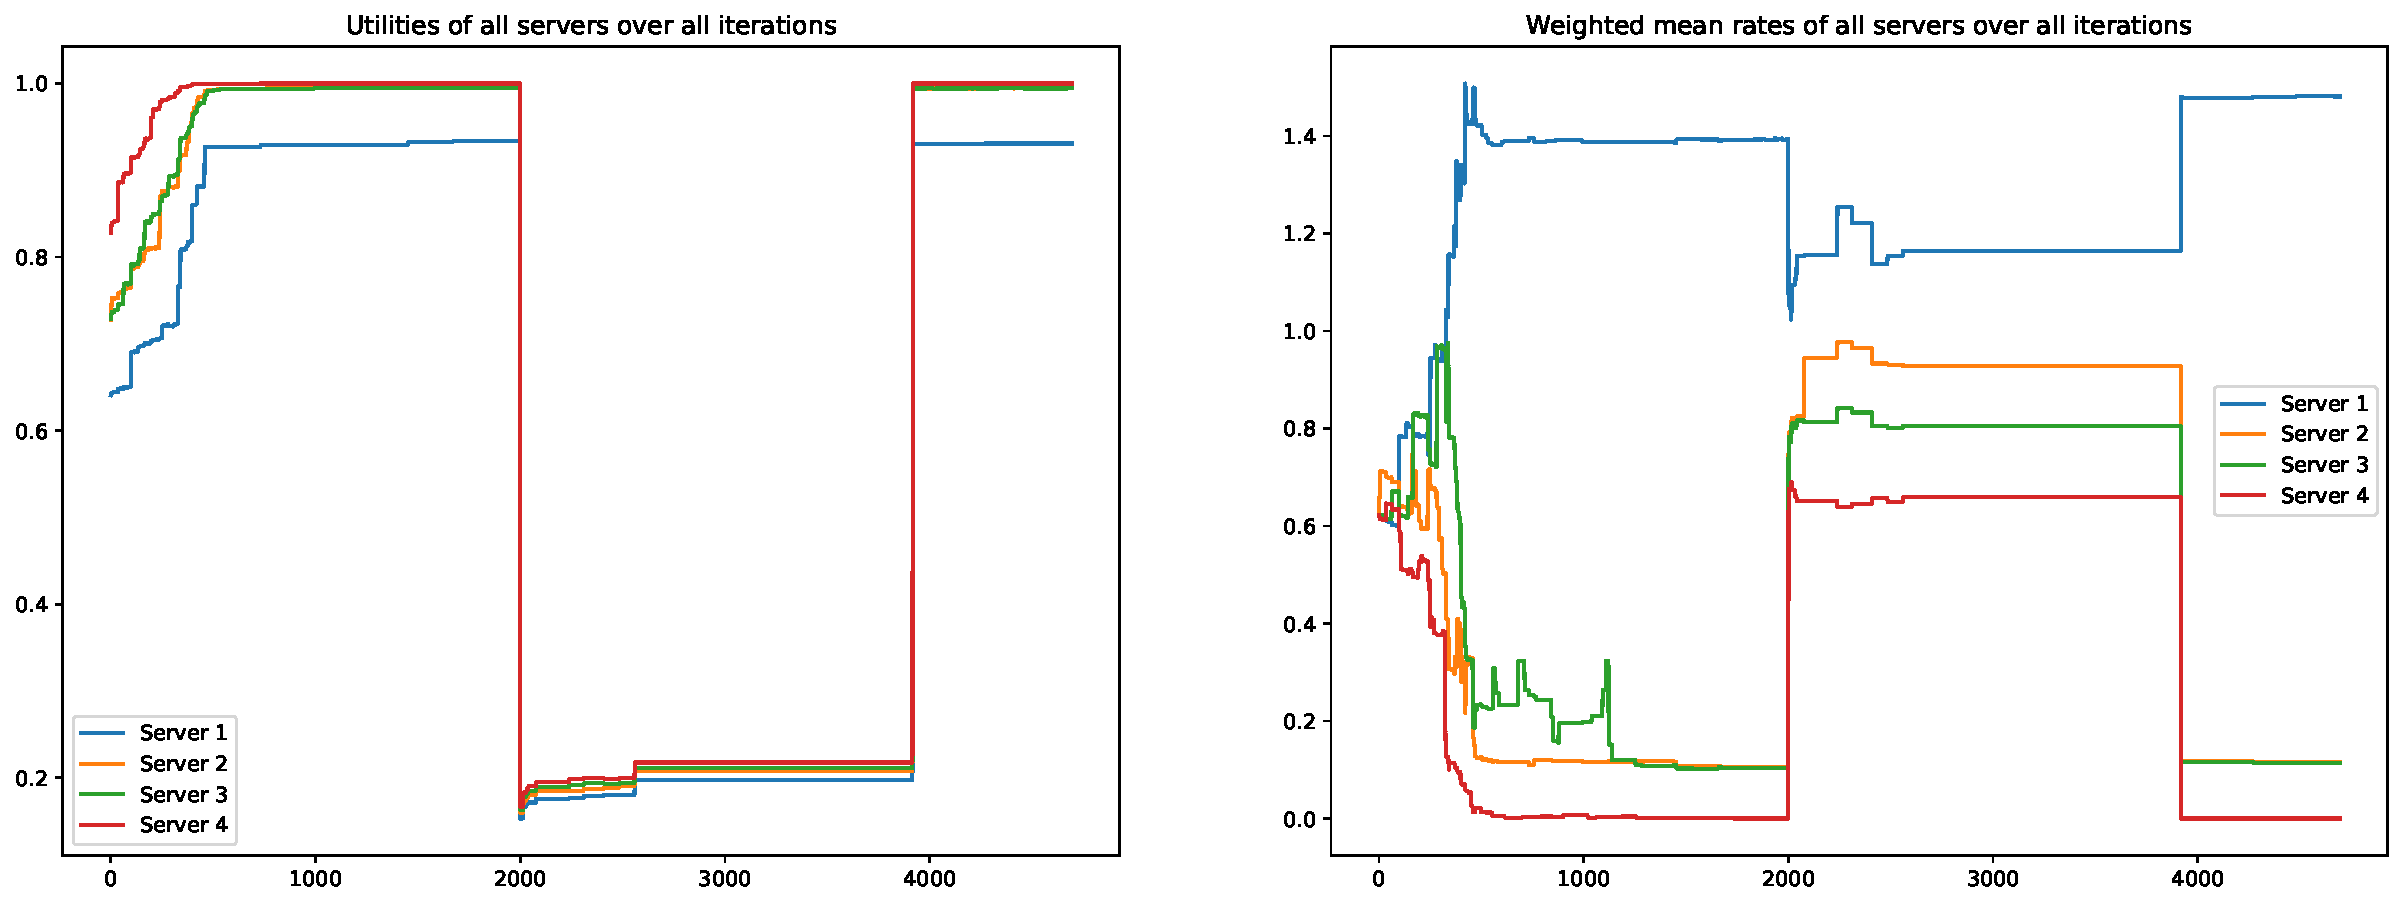
\includegraphics[width=\textwidth]{chapters/06_agent_based_extension/Bin/reinforcement_learning_results/utility_7/u7_6_final.pdf}
    \caption{Utilities (left) and weighted mean service rate (right) of servers
    from the reinforcement learning run using utility function \(U_k^{(7)}\)
    with \(e = 0.5\) and changing arrival rates throughout the run.}
    \label{fig:RL_utility7_6_final}
\end{figure}

Figure~\ref{fig:RL_utility7_6_final} shows the utilities and the weighted mean
service rates of the servers.
The first \(2000\) time steps are identical with the first \(2000\) time steps
of the reinforcement learning run of Figure~\ref{fig:RL_utility7_4_e05}.
At time step \(2000\), when the arrival rates are increased to \(\lambda_1 = 3\)
and \(\lambda_2 = 3.5\), the utilities of the agents drop significantly.
At the same time the weighted mean service rates of servers \(2\), \(3\) and
\(4\) increase significantly while server \(1\)'s rates are decreased.
In other words the arrival rates are increased so much that the priority of
the servers does not matter that much anymore.
All servers are constantly busy an they end up having more similar service
rates with each other.

At time step \(4000\) the arrival rates are decreased back to \(\lambda_1 =
0.5\) and \(\lambda_2 = 1\).
The utilities of the agents increase again and the weighted mean service rates
of servers \(2\), \(3\) and \(4\) decrease while server \(1\)'s rates are
increased.
What is more important here is how the utilities and the weighted mean service
rates change.
Having learned their optimal service rates during the first \(2000\) time steps
the servers are able to quickly retrieve their chosen service rates when the
arrival rates are decreased back to \(\lambda_1 = 0.5\) and \(\lambda_2 = 1\).
